\chapter{\TitreChapitreSix}\label{chap:Imagerie}

\bfigh
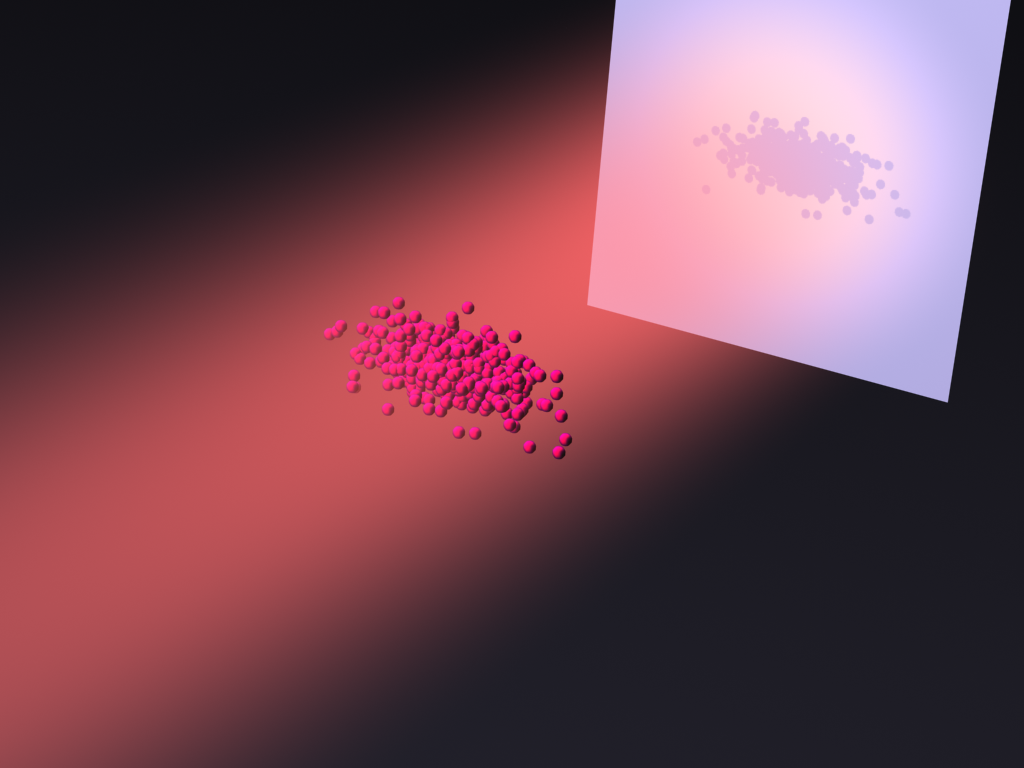
\includegraphics[width=\FigWidth]{P3/ChapitreImagerie}
\SansCaption
\efigh

\pagebreak

\minitoc
\vspace{0.5cm}

\noindent Lorsque l'on manipule des atomes froids, il est primordial de pouvoir caractériser les ensembles atomiques mis en jeu.
Les quantités physiques auxquelles nous voulons avoir accès sont le plus souvent:
\begin{itemize}
	\item le nombre d'atomes,
	\item la distribution spatiale des atomes dans le nuage,
	\item la distribution de vitesse,
	\item la \ddedpup.
\end{itemize}
Les techniques qui permettent d'acquérir ces informations sont quasi-exclusivement de nature optique, \cad se basant sur des processus d'absorption, de diffusion, ou de déphasage d'une onde lumineuse%
%
%\footnote{Mentionnons un exemple de technique non optique développée par le groupe d'Alain Aspect (institut d'optique, Orsay): Les atomes d'un \bec d'atomes d'hélium méta-stables sont lâchés en chute libre sur un capteur matriciel. Certains atomes d'hélium méta-stables délivrent une énorme énergie électrique ($\approx 20$ eV) en se désexcitant au contact du capteur. En mesurant précisément les temps et position d'arrivée sur le capteur, il est possible de construire une image en trois dimension de la distribution spatiale au sein du \bec. Il est même possible d'observer l'analogue atomique de l'effet Hanbury Brown Twiss~\cite{SHP05}.}.

Dans ce chapitre, nous allons décrire les deux principales méthodes couramment utilisées pour produire des images d'ensembles atomiques ultra-froids : l'\termetech{\ipf} et l'\termetech{imagerie par absorption dans le régime de faible saturation}. Les limites de ces méthodes, quand il s'agit de produire des images de \ns denses, nous amèneront à nous pencher sur des techniques plus élaborées, mais plus complexes à mettre en \oe uvre. 
%Nous avons ainsi été amenés à développer une nouvelle méthode d'imagerie par absorption. Cette dernière exploite la réponse non-linéaire des atomes lorsqu'ils sont soumis à un laser résonnant fortement saturant. J'ai contribué à l'élaboration puis à la mise en \oe uvre d'un protocole de mesure fiable pour ce nouveau type d'imagerie. Nous l'avons utilisé de manière systématique pour l'étude du piège magnéto-optique comprimé. Cette méthode étant remarquablement robuste, nous espérons que nos travaux contribueront à en populariser l'utilisation dans notre communauté. 
Enfin, nous présenterons le nouveau protocole d'imagerie que nous avons développé lors de ma deuxième année de thèse. Celui-ci permet de résoudre les structures de \nats denses et donne accès à des mesures quantitatives et précises.

\casse

\section{Imagerie d'un ensemble atomique froid}\label{sec:FaireLimage}
Dans cette section, nous allons décrire un dispositif optique minimal, qui nous permettra d'introduire les notions nécessaires à l'étude de l'imagerie d'un ensemble atomique. Nous porterons notre attention sur la nature numérisée de l'information obtenue lors d'une prise d'image. Les interactions atome-laser seront aussi décrites, puisque les équations qui en découlent permettent d'exploiter de manière quantitative les données contenues dans une image.


\subsection{Système optique}\label{sec:SystOptique}
Afin de concentrer notre attention sur le principe des méthodes d'imagerie, nous considèrerons le dispositif le plus simple possible en négligeant les imperfections des composants optiques%
\footnote{Nous négligerons donc les imperfections comme l'astigmatisme, les aberrations sphériques, etc.}%
. Nous supposerons être dans le cadre de l'approximation de Gauss. 
L'axe optique sera pris comme étant l'axe $z$. 
La figure~\nref{fig:SytemeOptique} représente un système optique simple permettant de produire l'image du \nat sur un capteur CCD composé d'une matrice de pixels. Nous pouvons ainsi mesurer la répartition d'intensité lumineuse $\Ixy$ provenant du plan objet%
%
\footnote{CCD est l'acronyme anglais de \termetech{Charge-Coupled Device} qui signifie \termetech{détecteurs à couplage de charge}. Ce type de capteur fournit un signal électrique dont la tension est proportionnelle à \emph{l'énergie lumineuse} collectée pendant le temps d'exposition $\texpo$. Connaissant ce temps, l'efficacité de détection et la surface représentée par un pixel dans le plan objet, nous pouvons déduire l'intensité lumineuse de la lumière qui a atteint chaque pixel.}%
.
%\subsubsection{aezaezaezaeaeaea}
%Certaines conditions doivent être réunies afin que le système optique puisse fournir des images exploitables. En particulier, la taille du nuage suivant l'axe $z$ sera supposée très faible par rapport à la \termetech{profondeur de champ} du système optique. En d'autres termes, dans l'approximation de Gauss, 
%\RemarqueTitre{Profondeur de champ}
%{
%}
\bfighs
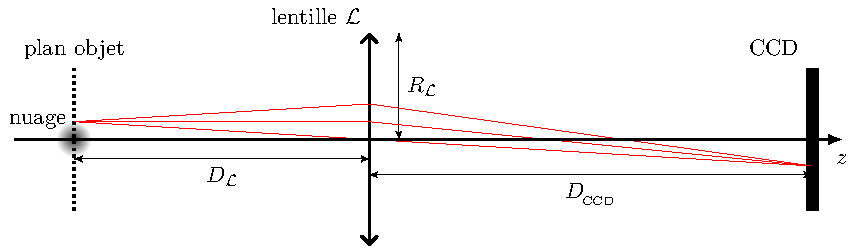
\includegraphics[scale=1]{P3/SytemeOptique}
\CaptionFigssss{Schéma représentant un système optique simple. Le plan objet, conjugué du capteur CCD se situe au niveau du nuage. Un point $(x',y')$ du capteur correspond à un point $(x,y) = (\ttfrac{x'}{\Grandis},\ttfrac{y'}{\Grandis})$ du plan objet, où $\Grandis=\ttfrac{\LentilleCCD}{\NuageLentille}$ est le grandissement du système optique.}
\label{fig:SytemeOptique}
\efigh

{\AjouteLigne}

Dans toute la suite, nous considèrerons un \nat dont la \dat sera notée $\densxyz$. Ce \n est situé au niveau du plan objet de système optique, et nous supposerons que chaque point $\xyz$ du nuage possède un point image en $(x',y')$ sur le capteur CCD. 
Ceci implique que le système n'est pas sensible à la position $z$ des atomes, mais uniquement à leur position $\xy$, projetée sur le plan objet.%
\nome{\denscol}{Densité colonne d'atome intégrée selon l'axe $z$}%{2cm}% 
%Le grandissement de ce système optique, $\Grandis=\ttfrac{\LentilleCCD}{\NuageLentille}$, définit la relation entre les bases $\xy$ et $(x',y')$ : un point $(x',y')$ du capteur correspond à un point $(x,y) = (\ttfrac{x'}{\Grandis},\ttfrac{y'}{\Grandis})$ du plan objet.
%
\Resultat
{
L'existence de cet axe privilégié d'observation, nous conduira par la suite à considérer la \emph{\dcol} $\denscolxy$ définie par:%
%\RemonteUnPeuFig
\begin{equation}
	\denscolxy \equiv \Integrale{\densxyz}{\dz}
	\pointformule
%\RemonteUnPeuFig
	\label{eq:denscol}
\end{equation}
Celle-ci correspond à la densité surfacique d'atomes si le nuage était projeté sur le plan $\xy$. Obtenir une image du \n consistera à mesurer cette grandeur.
}
Il est clair que la connaissance de la \dcol $\denscolxy$ ne suffit pas à déterminer la \dat $\densxyz$ du \n. Cette ambigüité de la mesure peut être levée en supposant que le \n possède certaines symétries.

\subsubsection{Échantillonnage spatial}
	Le nombre fini de pixels sur le capteur fixe une limite quant à la précision spatiale du signal fourni par le CCD. C'est ce qu'on appelle l'\emph{échantillonnage spatial} (aussi désigné par le terme \emph{pixelisation}). Pour les capteurs CCD usuels, la taille d'un pixel est typiquement de l'ordre de $\Lpix=\micron{5}$%
\footnote{Le capteur CCD utilisé sur notre \setup est un modèle \textbf{Basler A102 f} monochrome. La dimension des pixels est de $\micron{6.45} \times \micron{6.45}$. 
}%
. Cette limitation est à prendre en compte quand on désire faire des images d'ensembles atomiques dont l'extension spatiale est très faible (typiquement inférieure à \micron{100}). Le système optique devra alors être conçu de manière à fournir une image agrandie du nuage sur le capteur. 
	
\noindent Dans la suite, nous négligerons cet aspect. Par ailleurs, le signal fourni par la matrice du capteur sera noté $\Signal\xy$, où $\xy$ correspondra aux coordonnées \emph{dans le plan objet du \nat}.



\subsubsection{Système laser}%\label{sec:ImagerieLaser}
Sauf mention contraire, le système laser que nous considèrerons dans la suite est schématisé sur la figure~\nref{fig:SystemeLaser}.
Nous pouvons produire des impulsions lumineuses dont la durée $\TPulse$, et la puissance $\PLaser$ sont contrôlées précisément. Les impulsions les plus courtes que nous utilisons avec notre système ont une durée $\TPulse = \nanos{250}$.
\bfigh
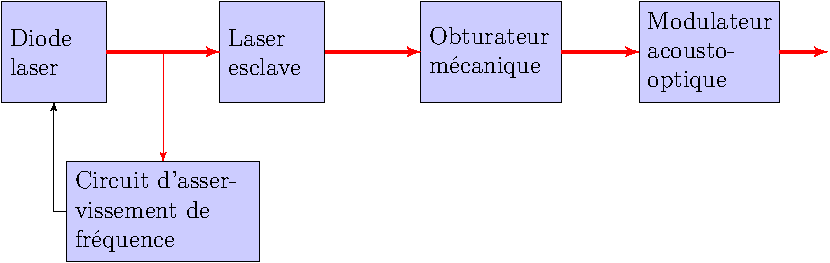
\includegraphics[scale=1]{P3/SystemeLaser}
\CaptionFigs{Schématisation d'un système laser simple. Une diode laser est verrouillée en fréquence grâce à un circuit d'asservissement. Les fluctuations de fréquence ainsi obtenues doivent être très faibles devant la largeur spectrale naturelle $\pulsSpont$ du \Rb. On peut typiquement espérer une puissance utilisable de quelques milliwatts. Pour disposer de plus de puissance, une seconde diode laser (\emph{esclave}), plus puissante, peut être \emph{injectée} par le premier faisceau et délivrer alors quelques dizaines de milliwatts. Un modulateur acousto-optique permet de produire des impulsion lumineuses de durée et de puissance contrôlées. 
Afin de s'affranchir des inévitables fuites de lumière à travers le modulateur, un obturateur mécanique est utilisé pour couper le faisceau durant les périodes d'inutilisation.}
\label{fig:SystemeLaser}
\efigh


\casse

\subsubsection{Utilisation du capteur CCD comme puissance-mètre}
Mentionnons un dernier point quant à l'interprétation du signal fourni par le capteur CCD. Dans les conditions de fonctionnement normal, chaque pixel fournit un signal $\Signal$ proportionnel à l'énergie lumineuse $\Epix$ accumulée pendant le temps d'exposition $\TPulse$. Or, nous verrons dans la suite que l'information que nous exploitons en pratique est \emph{la répartition d'intensité} $\Ixy$ dans le plan objet du système optique (là où se trouve le nuage). Le capteur CCD peut tout à fait fournir cette information si l'on connait les paramètres suivants :
\begin{itemize}
	\item la sensibilité du capteur,
	\item le grandissement $\Grandis$ %
	\nome{\Grandis}{Grandissement du système optique}%
	du système optique qui détermine la surface que représente un pixel dans le plan objet,
	\item la durée $\TPulse$ %
	\nome{\TPulse}{Durée du pulse du faisceau imageur}%
	d'exposition qui détermine la puissance lumineuse reçue,
	\item les pertes et atténuations $\AttenOptique$ sur le trajet du faisceau dans le système optique, entre le plan objet et le capteur.
\end{itemize}
Nous désignerons par $I'\xpyp$ la répartition d'intensité mesurée sur le capteur. L'intensité $\Ixy$ dans le plan objet se déduit alors par l'expression:%
\nome{\Ixy}{Intensité lumineuse dans le plan objet}%
\begin{equation}
	\Ixy = \AttenOptique \, \Grandis^2 \, I'(\Grandis\,x,\Grandis\,y)
	\label{eq:ICCD}
\end{equation}
Dans toute la suite de ce chapitre, les signaux provenant du capteur CCD seront systématiquement interprétés \emph{en terme d'intensité $\Ixy$ dans le plan objet}.
\Resultat{
Cependant, afin de souligner le caractère expérimental de cette grandeur mesurée par le capteur CCD, nous utiliserons la notation $\Iccdxy$ pour désigner l'intensité $\Ixy$ observée dans le plan objet où se situe le \nat.
}


\subsection{Interaction atome-laser}\label{sec:interAtomeLaser}
Afin d'interpréter les données acquises par des méthodes optiques, il est primordial de connaître les processus d'interaction entre les atomes et le champ électromagnétique.
La description détaillée de ces processus sort du cadre de ce manuscrit. Cependant, nous allons rappeler quelques notions élémentaires dans le cas simple d'un atome à deux niveaux en interaction avec une onde lumineuse monochromatique cohérente.
Le cas, expérimentalement pertinent, d'un atome ayant une structure énergétique complexe est abordé dans la~\autoref{sec:ipafos}.

{\AjouteLigne}

\subsubsection{Modélisation par atome à deux niveaux d'énergie}
%\vspace{-1cm}
\inlinefig{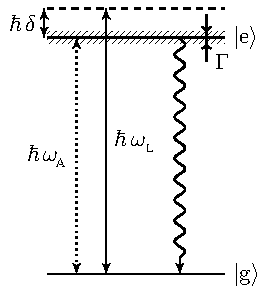
\includegraphics{P3/EnergieAtome2Niveaux}}
%Rappelons les notations nécessaires à l'étude de l'imagerie
Nous examinons ainsi l'interaction entre les atomes du nuage et la lumière monochromatique d'un laser de pulsation $\pulsLaser$%
\nome{\pulsLaser}{Pulsation du laser imageur}%
. Nous considérons le cas simple d'un \emph{atome à deux niveaux d'énergie}: l'état \emph{fondamental} par $\EtatG$ et l'état \emph{excité} $\EtatE$. L'énergie $\energieGE$ qui sépare ces deux niveaux correspond à une pulsation de résonance
$
\pulsReso = \ttfrac{\energieGE}{\hbar}
%\virguleformule
$.%
\nome{\pulsReso}{Pulsation de résonance de l'atome à 2 niveaux}%
%pour la transition \TransGE. 
Cette transition possède une largeur spectrale naturelle $\pulsSpont$ liée à la durée de vie $\tSpont$ du niveau excité. Le désaccord entre la pulsation laser $\pulsLaser$ et la pulsation $\pulsReso$ de résonance sera noté $\desac$ %
\nome{\desac}{Désaccord entre la pulsation laser $\pulsLaser$ et la pulsation $\pulsReso$ de résonance}%:
\[
\desac \equiv \pulsLaser - \pulsReso
\pointformule
\]
\picskip{0}

\casse


\RemarqueTitre{Élargissement inhomogène}{
Nous négligerons dans toute la suite les sources d'élargissement inhomogène, \cad que nous considèrerons que les atomes du \n réagissent tous de la même manière vis à vis de la lumière. La pulsation de résonance $\pulsReso$ est ainsi la même pour tous les atomes. Ceci suppose en particulier que:
\begin{itemize}
	\item la température du nuage soit faible devant la température Doppler afin de s'affranchir de l'effet Doppler.	Pour le \Rb, $\TDoppler \approx \microK{146}$.
	\item il n'y ait pas de gradient de \chm notable sur l'extension spatiale du \n.
\end{itemize}
De manière plus générale, tout type de confinement (magnétique, dipolaire, etc) déplaçant les niveaux énergétiques des atomes, devra être coupé lors de la prise d'images. Ceci signifie que le nuage est alors en expansion balistique.
}

\subsubsection{Équations de Bloch optiques}
Rappelons simplement que, dans le cas considéré ici d'une onde lumineuse cohérente agissant sur un système à deux niveaux, il est possible de décrire l'évolution des populations et des cohérences atomiques grâce aux \termetech{\EBO}%
\footnote{Nous supposerons dans toute la suite que la distance moyenne entre atomes est supérieure à la longueur d'onde du laser, sans quoi des effets \termetech{collectifs} peuvent intervenir et le formalisme des \EBO ne serait plus adapté.}%
. Celles-ci s'obtiennent en effectuant plusieurs approximations que nous rappelons ici:
\begin{itemizel}
	\item l'approximation du \termetech{champ tournant}
	\footnote{Cette approximation consiste à négliger les grandeurs oscillant à des fréquences très élevées (le double de la fréquence optique) et dont les valeurs moyennes sont nulles.},
	\item l'approximation de \termetech{mémoire courte}
	\footnote{Celle-ci consiste à considérer que les modes vides du rayonnement électromagnétique constituent un \sotosay{réservoir} dont les fluctuations sont extrêmement rapides. Ceci assure en particulier que l'émission spontanée est un phénomène irréversible.},
	\item il faut aussi supposer que toutes les fréquences typiques de couplage entre atome et champ sont négligeables devant la fréquence optique
	\footnote{Ceci revient à supposer que la pulsation de Rabi, le taux d'émission spontanée $\pulsSpont$ du niveau excité, et le désaccord  $\desac$ sont négligeables devant $\pulsLaser$. Cette approximation est en générale très bien vérifiée dans le domaine optique%, mais peut être mise à défaut si on utilise des champs lasers impulsionnels extrêmement intenses
.}.
\end{itemizel}
%
Dans toute la suite, nous considèrerons \emph{le régime stationnaire}%
%
\footnote{Les \EBO montrent que la constante de temps typique d'établissement du régime stationnaire est $\tfrac{1}{\pulsSpont}\approx \nanos{26}$ dans le cas du \Rb. Avec les impulsions lumineuses que nous utilisons en pratique (d'une extension temporelle allant typiquement de \micros{0.5} à \micros{100}), le régime stationnaire représente l'essentiel de la dynamique d'interaction.}
%
 atteint par un atome soumis à une onde laser d'intensité $\Ilaser$, désaccordée de $\desac$.  
\noindent Dans ce cas, la population $\PopuE$ de l'état excité est donnée par %
\nome{\PopuE}{Population atomique de l'état excité}%
:
\begin{equation}
	\PopuE = \frac{1}{2}\,\frac{\sat}{1+\sat}
	\virguleformule
	\label{eq:PopuEParamSat}
\end{equation}
où $\sat$ est le \emph{paramètre de saturation} de la transition. Il est proportionnel à l'intensité laser $\Ilaser$, et dépend du désaccord $\desac$ suivant une loi lorentzienne %
\nome{\sat}{Paramètre de saturation de la transition atomique}%
:
\begin{equation}
	\sat \equiv \IsurIsat  
	\, \left. \frac{1}{ 1 + \left(\dfrac{2\,\desac}{\pulsSpont}\right)^2 } \right. 
	\pointformule
	\label{eq:ParamSat}
\end{equation}

\casse

\ifthenelse{\FormatEUE > 0}{}
{\AjouteLigne}

\noindent
$\Isat$ désigne \emph{\lintsat à résonance}, qui correspond à la valeur de l'intensité du laser à résonance, pour avoir $\PopuE = \ttfrac{\PopuEmax}{2} = \tfrac{1}{4}$. 
Elle s'exprime simplement en fonction du taux d'émission spontanée dans le cas d'un atome à deux niveaux %
\nome{\Isat}{Intensité de saturation à résonance}%
:
\begin{equation}
	\Isat = \frac{2\,\pi^2\,\hbar\,c\,\pulsSpont}{3\,\lambda^3}
	\pointformule
	\label{eq:IsatExpr}
\end{equation}
\RemarqueTitre{Effet de saturation}{\RemonteUnPeuFig
\inlinefig{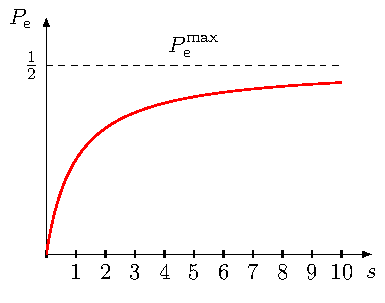
\includegraphics{P3/CourbeSat}}
Notons que la population dans l'état excité est une \emph{fonction non-linéaire de l'intensité $\Ilaser$} (voir la figure ci-contre):
\[
\PopuE\xrightarrow[\Ilaser \rightarrow \infty]{~~~~~~~~~~~~~}\PopuEmax = \tfrac{1}{2}
\]
Cet effet de saturation est de nature purement quantique. Il est lié au fait qu'un atome peut émettre un photon de manière stimulée depuis son état excité $\EtatE$, et ce avec la même probabilité qu'il a d'en absorber un depuis son état fondamental $\EtatG$.
\picskip{2}\vspace{-0.5cm}
}

Dans la suite de ce chapitre, et sauf mention contraire, nous considèrerons implicitement une onde laser ayant un désaccord nul : $\desac=0$. Nous préciserons les raisons de ce choix dans la~\autoref{sec:ImagerieDesaccordee}.


\subsection{Absorption et diffusion de la lumière au sein d'un \nat} \label{sec:PuissanceDiffusee}
Nous allons maintenant considérer un ensemble atomique de \dat $\densxyz$ soumis à une onde laser dont la répartition d'intensité est $\Ixyz$. 
Nous allons exprimer la puissance lumineuse absorbée et diffusée au sein du \n. Les relations qui seront obtenues dans cette sous-section seront utilisées dans la suite de ce chapitre.
%Nous supposerons dans tout la suite qu'il n'y a pas d'effets collectifs, \cad que chaque atome se comporte indépendamment des autres.
\Remarque{
Le paramètre $\sat$ est proportionnel à l'intensité laser $\Ixyz$ et dépend donc des coordonnées $\xyz$. Cependant, pour alléger les expressions, nous conserverons la notation $\sat$ pour exprimer $\sat\xyz$.
}

%\subsubsection{Puissance lumineuse absorbée et diffusée au sein du \nat}
Chaque atome absorbe et diffuse%
%
\footnote{En régime stationnaire, la \popuexcit est constante, ce qui traduit le fait qu'il y a en moyenne autant de photons absorbés que de photons diffusés.}%
,
 un nombre moyen $\pulsSpont\,\PopuE$ de photons par unité de temps. En chaque point \xyz du \n (dont la \dat est $\densxyz$), la puissance $\Diff{\Pdif}$ absorbée et diffusée dans un volume élémentaire $\dxyz$ est donc donnée par %
 \nome{\Pdif}{Puissance lumineuse absorbée et diffusée au sein du \nat}%
 :
\nResultat{%
\begin{align}
	\Diff{\Pdif} & = \hbar\,\pulsReso\,\pulsSpont\,\PopuE \, \dens\,\dxyz \nonumber \\
	& = \hbar\,\pulsReso\, \pulsSpont \, \frac{1}{2} 
%	\, \IsurIsatxyz 
%	\, \frac{1}{1 + \IsurIsatxyz + \left(\dfrac{2\,\desac}{\pulsSpont}\right)^2}
	\, \frac{\sat}{1+\sat}
	\, \densxyz\,\dxyz 
	\virguleformule
	\label{eq:Pdif}
\end{align}
}
\nRemarque{Notons que l'expression~\nref{eq:Pdif} ne fait intervenir aucune hypothèse sur la répartition spatiale de l'intensité laser $\Ixyz$ au sein du \n. Cette expression est par exemple valable, que ce soit pour une onde progressive traversant le nuage, ou encore pour une onde stationnaire produite par un ensemble de faisceaux lasers.
}



\EnFaitNon
{%%%%%%%%%%%%%%%%%%%%%%%%%%%%%%%%%%%%%%%%%%%%%%%%%%%%%%%%%%%%%%%%%%%
%%%%%%%%%%%%%%%%%%%%%%%%%%%%%%%%%%%%%%%%%%%%%%%%%%%%%%%%%%%%%%%%%%%
%%%%%%%%%%%%%%%%%%%%%%%%%%%%%%%%%%%%%%%%%%%%%%%%%%%%%%%%%%%%%%%%%%%
%%%%%%%%%%%%%%%%%%%%%%%%%%%%%%%%%%%%%%%%%%%%%%%%%%%%%%%%%%%%%%%%%%%
\subsubsection{Utilisation d'un faisceau laser peu saturant}

Si l'intensité $\Ixyz$ est faible devant \lintsat $\Isat$, ou encore si le désaccord $\desac$ est , \ie $\sat \ll 1$, l'expression~\nref{eq:Pdif} devient:
\begin{align}
	\Diff{\Pdif} & =
	\sat
	\, \frac{\hbar\,\pulsReso\,\pulsSpont}{2} 
	\, \densxyz\,\dxyz
	\,\,\,\,\, \mbox{avec} \,\,\, \sat \ll 1
	\nonumber \\
	& = 
	\Ixyz
%	\, \frac{\hbar\,\pulsReso\,\pulsSpont}{2\,\Isat} 
%	\, \frac{1}{1 + \left(\dfrac{2\,\desac}{\pulsSpont}\right)^2}
	\, \frac{\seceff}{1 + \left(\dfrac{2\,\desac}{\pulsSpont}\right)^2}
	\, \densxyz\,\dxyz
	\pointformule
	\label{eq:PdifBasseInt}
\end{align}
Dans cette limite, la puissance absorbée et diffusée $\Pdifxyz$ et proportionnelle à la \dat locale $\densxyz$, \emph{et} à l'intensité lumineuse locale $\Ixyz$.

\subsubsection{Utilisation d'un faisceau laser très saturant}
Si l'intensité $\Ixyz$ est grande devant \lintsat $\Isat$, \ie $\sat \gg 1$, l'expression~\nref{eq:Pdif} devient:
\begin{align}
	\Diff{\Pdif} & =
	\, \frac{\hbar\,\pulsReso\,\pulsSpont}{2} 
	\, \densxyz\,\dxyz
	\,\,\,\,\, \mbox{avec} \,\,\, \sat \ll 1
	\nonumber \\
	\pointformule
	\label{eq:PdifHauteInt}
\end{align}
Dans cette limite, la puissance absorbée et diffusée $\Pdifxyz$ et alors proportionnelle à la \dat $\densxyz$, mais est indépendante de l'intensité lumineuse locale $\Ixyz$.
%%%%%%%%%%%%%%%%%%%%%%%%%%%%%%%%%%%%%%%%%%%%%%%%%%%%%%%%%%%%%%%%%%%
%%%%%%%%%%%%%%%%%%%%%%%%%%%%%%%%%%%%%%%%%%%%%%%%%%%%%%%%%%%%%%%%%%%
%%%%%%%%%%%%%%%%%%%%%%%%%%%%%%%%%%%%%%%%%%%%%%%%%%%%%%%%%%%%%%%%%%%
%%%%%%%%%%%%%%%%%%%%%%%%%%%%%%%%%%%%%%%%%%%%%%%%%%%%%%%%%%%%%%%%%%%
}

\casse

\section{Fiabilité d'une prise d'image}\label{sec:precautions}

Les protocoles de mesures décrits dans la section suivante correspondent le plus souvent à des mesures destructives, \cad modifiant les propriétés du nuage dont l'image est faite. En effet, l'absorption et la diffusion de photons, fait évoluer les propriétés du \nat (taille, température,\ldots).
Pour cette raison, il est souvent impossible de pratiquer deux mesures successives sur un même nuage. 
\Remarque{
Dans la suite (notamment dans la~\autoref{sec:ipafos}), quand nous proposerons de faire plusieurs fois l'image d'un même nuage, il faudra garder à l'esprit que chaque mesure est en fait effectuée sur un \nat \emph{différent}, mais préparé rigoureusement dans les \emph{mêmes conditions expérimentales}. Une bonne \emph{reproductibilité de l'expérience} est alors une condition \textit{sine qua non}, afin d'assurer la production répétée de nuages identiques.
}

%Nous pouvons donc nous accommoder du fait que la mesure modifie les propriétés du nuage. Toutefois, 
Il est de plus primordial que les propriétés du \nat ne changent pas de manière significative \emph{pendant} la prise d'une image, sans quoi l'image n'est plus exploitable. Sur ce point, nous nous proposons dans cette section de discuter la fiabilité d'une prise d'image, dans le cas simple d'une impulsion laser de durée $\TPulse$ éclairant un nuage. Nous supposerons pour simplifier que le paramètre de saturation $\sat$ est le même pour chaque atome du nuage.

\subsection{Diffusion due à l'agitation \thiq}\label{sec:FiabilitéImageThiq}
Avant de considérer l'effet de la lumière sur les degrés de liberté externes des atomes, rappelons que, dans la plupart des cas rencontrés, le confinement du nuage est coupé au moment de la prise d'image. L'\emph{expansion balistique} du nuage pendant la prise d'image doit être considérée. En effet, si on considère un nuage à l'\eqthdy défini par la température $T$, la vitesse quadratique moyenne des atomes au sein du nuage est $\Dv=\sqrt{\ttfrac{\kb\,T}{m}}$. Chaque atome se déplace en moyenne%
\footnote{Ce raisonnement suppose l'absence d'interactions inter-atomiques pendant la durée $\TPulse$ de l'impulsion lumineuse. Cependant, $d=\TPulse\,\Dv$ reste une borne supérieure pour la distance moyenne parcourue par un atome.}
 de $d=\TPulse\,\Dv$ pendant la durée $\TPulse$ de l'impulsion. La distance $d$ est donc une borne supérieure quant à la résolution spatiale que l'on peut espérer lors de la prise d'image.
\ApplicationNumerique{
Considérons un nuage dont la température d'\eqthdy est $T=\microK{100}$. Calculons la durée maximale $\TPulse$ qui soit compatible avec une diffusion des positions atomiques inférieure à $d=\micron{10}$ (ceci correspond à la taille typique $\Lpix$ représenté par un pixel du capteur CCD dans le plan objet):
\begin{equation}
\TPulse \leqslant d\,\sqrt{\frac{m}{\kb\,T}} \approx \micros{100}
\pointformule
	\label{eq:tauTemp}
\end{equation}
Si cette condition est vérifiée, chaque atome contribue, en moyenne, au plus à un pixel sur le capteur CCD.
}

\casse

\subsection{Accélération due à la pression de radiation}
Le premier effet du laser sur la position et la vitesse des atomes est la pression de radiation. Celle-ci pousse les atomes dans le sens de propagation de l'onde laser. D'après l'expression~\nref{eq:Pdif}, chaque atome absorbe (puis diffuse dans une direction aléatoire) en moyenne  un nombre 
$\tfrac{\pulsSpont}{2}\,\tfrac{\sat}{1+\sat}$
de photons par unité de temps. Ceci correspond à une accélération moyenne $a$, une vitesse moyenne $v_\TPulse$ et un déplacement spatial moyen $d_\TPulse$ à la fin de l'impulsion de durée $\TPulse$:
\[
	a = \vrecul \, \frac{\pulsSpont}{2}\,\frac{\sat}{1+\sat}
\virguleformule
\qquad
	v_\TPulse = \TPulse \, \vrecul \, \frac{\pulsSpont}{2}\,\frac{\sat}{1+\sat} 
\virguleformule
\qquad
	d_\TPulse = \TPulse^2 \, \vrecul \, \frac{\pulsSpont}{4}\,\frac{\sat}{1+\sat} 
\virguleformule
\]
où $\vrecul = \tfrac{\hbar\,k}{m} = \tfrac{\hbar\,\pulsReso}{m\,c}$ est la vitesse de recul de l'atome ($\approx\mmps{6}$ pour le \Rb).

\noindent De manière à produire une image exploitable, il est préférable de ne pas trop accélérer les atomes pendant la prise d'image, sans quoi l'effet Doppler modifie le désaccord apparent du laser: $\desac \rightarrow \desac + k\,v_\TPulse$.
\ApplicationNumerique{
Quelle condition doit-on remplir pour avoir un déplacement par effet Doppler négligeable devant la largeur naturelle $\pulsSpont$ de la transition? Nous pouvons écrire:
\RemonteUnPeuFig
\[
v_\TPulse\,\frac{2\,\pi}{\lambda} \ll \pulsSpont
\virguleformule
\RemonteUnPeuFig
\]
où $\lambda$ est la longueur d'onde du laser. Nous obtenons donc la condition sur la durée $\TPulse$ de l'impulsion lumineuse et le paramètre de saturation $\sat$:
\RemonteUnPeuFig
\[
\TPulse \,\frac{\sat}{1+\sat} \ll \frac{\lambda}{\pi\,\vrecul} \approx \micros{40}
\pointformule
\RemonteUnPeuFig
\]
On pourra donc s'autoriser des impulsions lumineuses très intenses ($\sat \gtrsim 1$) dont la durée est de l'ordre de la microseconde. Pour une impulsion dont l'intensité est faible ($\sat \ll 1$), la durée $\TPulse$ peut être plus grande (quelques dizaines de micro-secondes pour une intensité $\Ilaser = \ttfrac{\Isat}{10}$).
}


\subsection{Chauffage dû à l'émission spontanée}
Le deuxième effet est lié aux ré-émissions des photons dans des directions aléatoires et tend à faire diffuser les vecteurs vitesses de chaque atome. Ceci se traduit par un échauffement du nuage. En reprenant les notations précédemment utilisées, nous exprimons le taux de chauffage du nuage pendant l'impulsion lumineuse:
\[
\Derive{T}{t} = \frac{\pulsSpont}{2}\,\frac{m\,\vrecul^2}{\kb} \, \frac{\sat}{1+\sat}
%\approx \frac{\sat}{1+\sat} \times \microKpmicros{6} 
\pointformule
\]
\EnFaitNon%
{
Nous pouvons estimer une borne supérieure à l'effet de l'échauffement dû au laser. 
En reprenant le critère~\nref{eq:tauTemp} précédemment établi entre la température $T$ du nuage et la durée $\TPulse$ de l'impulsion, nous pouvons utiliser la valeur maximale de la température atteinte (même si celle-ci augmente en fait progressivement pendant l'impulsion):
\begin{equation}
\TPulse \leqslant d\,\sqrt{\frac{m}{\kb\,
\left( T 
+ \TPulse\,\dfrac{\pulsSpont}{2}\,\dfrac{m\,\vrecul^2}{\kb} \, \dfrac{\sat}{1+\sat}
\right)}} 
\pointformule
	\label{eq:tauTempEchauf}
\end{equation}
}
\ApplicationNumerique{
Dans le cas du \rb, l'échauffement peut s'exprimer numériquement, en fonction du paramètre de saturation $\sat$:
\[
\Derive{T}{t} \approx \frac{\sat}{1+\sat} \times \microKpmicros{7} 
\pointformule
\]
Cet échauffement n'est pas problématique tant qu'il n'affecte pas significativement la distribution des atomes durant la prise d'image (voir la \autoref{sec:FiabilitéImageThiq}).
%La relation~\nref{eq:tauTempEchauf} se résout exactement, et, pour reprendre les valeurs précédemment utilisées ($T=\microK{100}$ et $d=\micron{10}$), nous obtenons $\TPulse \leqslant \micros{50}$.
}


\casse

\section{Techniques d'imagerie usuelles}\label{sec:ImagerieUsuelles}
Différentes techniques peuvent être utilisées afin d'obtenir une image représentative de la \dat du \n. Dans cette section, nous présentons les deux principales méthodes couramment utilisées, puis nous soulignerons les limites de celles-ci quand il s'agit de produire des images de \ns très denses.


\subsection{\Ipf}\label{sec:ipf}
La technique qui semble la plus simple à mettre en \oe uvre consiste simplement à \sotosay{éclairer} le \nat et à recueillir la lumière diffusée par celui-ci à travers le système optique. On parle d'\emph{\ipf}.
Comme le montre la figure~\nref{fig:OptiqueFluo}, le faisceau laser incident n'arrive pas suivant l'axe optique $z$ de manière à ne pas gêner la détection de la lumière diffusée par le nuage.
\bfigh
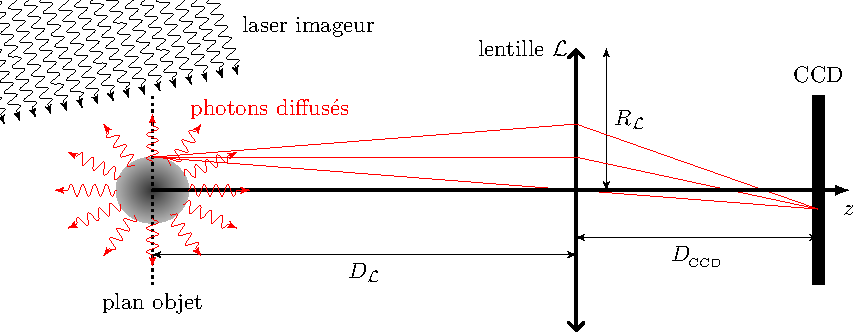
\includegraphics{P3/OptiqueFluo}
\CaptionFigssss{Schéma illustrant un système optique simple pour faire une image par fluorescence. Le faisceau laser incident n'arrive pas suivant l'axe optique $z$ de manière à ne pas gêner la détection de la lumière diffusée par le nuage. Nous avons représenté symboliquement l'émission spontanée de quelques photons. Seule une fraction de ceux-ci est émise en direction du système optique.}
\label{fig:OptiqueFluo}
\efigh

L'émission spontanée de photons est isotrope et seule une fraction de la lumière diffusée est recueillie par le système optique. Si $\RLentille$ est le rayon de la lentille et $\NuageLentille$ la distance nuage-lentille, celle-ci est \sotosay{vue} par le \n sous un angle solide %
\nome{\AngleSolide}{Angle solide d'interception de la lumière diffusée}%
:
\[
\AngleSolide = 2\,\pi\,\left( 1-\frac{\NuageLentille}{\sqrt{\RLentille^2+\NuageLentille^2}} \right)
\pointformule
\]
En supposant que tous les photons qui atteignent la lentille sont envoyés vers le capteur CCD, celui-ci mesure une fraction $\ttfrac{\AngleSolide}{4\,\pi}$ de la lumière diffusée par le nuage.
%
Le signal mesuré par le capteur CCD est donc% 
%\footnote{Rappelons que l'axe du système optique est l'axe $z$, $\Grandis$ est le grandissement du système optique, et $\AttenOptique$ est le facteur d'atténuation de la lumière entre le nuage est le capteur CCD (voir la~\autoref{sec:SignalCCD}).}
:
{\AjouteLigne}
\begin{equation}
	\Iccdxy 
	= \Ibackxy + \FractionAngleSolide \, \Integrale{{\Pdif\xyz}}{\dz} 
	\virguleformule
	\label{eq:IccdFluoPdif}
\end{equation} 
où $\Ibackxy$ désigne l'intensité de la lumière de fond%
\footnote{Cette lumière de fond provient de diverses sources, comme la lumière ambiante dans l'environnement du laboratoire, et qui atteint le capteur. La notation $\Iback$ se justifie par le terme conventionnel anglais, \termetech{background}, pour désigner la \termetech{lumière de fond}.}
qui est mesurée par le capteur CCD même en l'absence du nuage et ${\Pdif}$ est la puissance lumineuse diffusée par le nuage (voir la~\autoref{sec:PuissanceDiffusee}).
Notons que l'intégrale qui intervient dans l'expression~\nref{eq:IccdFluoPdif} traduit le fait que chaque point $\xyz$ du nuage possède une image en $\xy$ sur le capteur CCD. 


\subsubsection{Signaux mesurés par le capteur CCD}
\noindent
D'après l'expression~\nref{eq:Pdif} de la puissance diffusée au sein du \nat on peut écrire :
\begin{equation}
	\Iccdxy 
	=  \Ibackxy
	  + \FractionAngleSolide
	\, \frac{\hbar\,\pulsReso\,\pulsSpont}{2}
	\, \Integrale{\frac{\sat}{1+\sat} \, \densxyz}{\dz}
	\pointformule
	\label{eq:IccdFluo}
\end{equation} 
Cette relation fait intervenir l'intensité lumineuse locale $\Ixyz$ à travers le paramètre de saturation $\sat$. Or en pratique, cette intensité n'est pas uniforme dans l'espace pour deux raisons:
\begin{itemize}
	\item le profil transverse d'intensité du laser n'est jamais totalement uniforme,
	\item l'intensité du laser diminue au cours de sa propagation à travers le nuage.
\end{itemize}
Il est donc difficile, à partir du signal $\Iccdxy$, d'extraire une information quantitative sur la \dat $\densxyz$.
%
\Resultat{
En pratique, la technique usuelle d'\ipf consiste à considérer que le nuage entier est soumis à la même intensité lumineuse. On peut alors écrire la relation:
\begin{equation}
	\Iccdxy 
	\approx  \Ibackxy
	  + \FractionAngleSolide
	\, \frac{\hbar\,\pulsReso\,\pulsSpont}{2}\,\frac{\sat_0}{1+\sat_0}\,
	\, \denscolxy
	\virguleformule
	\label{eq:IccdFluoApprox}
\end{equation} 
où $\sat_0$ est un paramètre de saturation \sotosay{global} qu'il faut estimer en tenant compte du désaccord et de l'intensité lumineuse moyenne au niveau du \nat.
Le second membre de l'expression~\nref{eq:IccdFluoApprox} possède un terme proportionnel à la \dcol $\denscolxy$.
}
%
La figure~\nref{fig:ImagesFluo} représente une image d'un \n dans le \pmo décrit au chapitre~\nref{chap:JetAtomique}. 
%
\bfighs
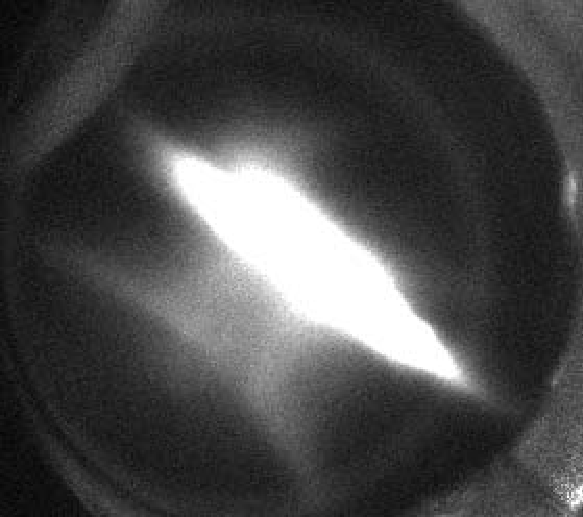
\includegraphics[width=6.5cm]{P3/FluoMotLoad_treslent0142}
\CaptionFigs{\Ipf prise lors du chargement du \pmo décrit dans le chapitre~\nref{chap:JetAtomique}. Typiquement \val{E9} atomes sont éclairés par les 6 faisceaux lasers du \pmo dont le désaccord est $\desac\approx-3\,\pulsSpont$.}
\label{fig:ImagesFluo}
\efigh

\casse

\noindent
Pour estimer le paramètre de saturation $\sat_0$ qui correspond à la figure~\nref{fig:ImagesFluo}, nous tenons compte des paramètres suivants:
\begin{itemize}
	\item 6 faisceaux lasers interviennent,% (deux à deux contrapropageant),
	\item leur intensité est d'environ $I\approx2\,\Isat$,
	\item le désaccord des faisceaux est $\desac\approx-3\,\pulsSpont$,
	\item nous négligeons l'inhomogénéité du \chm.
\end{itemize}
D'après l'expression~\nref{eq:ParamSat}, nous déduisons $\sat_0 \approx \val{0.3}$.


\subsubsection{Protocole de mesure pour l'\ipf}

L'expression~\nref{eq:IccdFluoApprox} contient donc un signal de fond $\Ibackxy$, et un signal utile, proportionnel à la \dcol. En pratique, on s'affranchit du premier terme en capturant non pas une, mais deux images sur le capteur CCD.
\begin{itemize}
	\item la première est une image du \nat, en présence de la lumière laser excitatrice; le signal recueilli correspond à l'expression~\nref{eq:IccdFluo}
	\item la deuxième est une image prise dans les mêmes conditions, \emph{mais en l'absence du nuage}; le signal mesuré est alors composé uniquement du terme $\Iccdxy = \Ibackxy$.
\end{itemize}
\Resultat{
Une simple soustraction des deux images permet d'obtenir un signal utile donnant la \dcol 
\[
\denscolxy = \frac{4\,\pi}{\AngleSolide}\,\frac{2}{\hbar\,\pulsReso\,\pulsSpont}\,
\left( 
\IccdxyAvecNuage - \IccdxySansNuage
\right) 
\pointformule
\]
}



\subsection{Imagerie par absorption dans le régime de faible saturation}\label{sec:ipafas}
L'autre méthode usuelle est l'\emph{imagerie par absorption}. Celle-ci consiste à éclairer le \nat avec une onde laser progressive et à faire l'image de son ombre (voir la figure~\nref{fig:OptiqueAbsorption}).
%
\bfighs
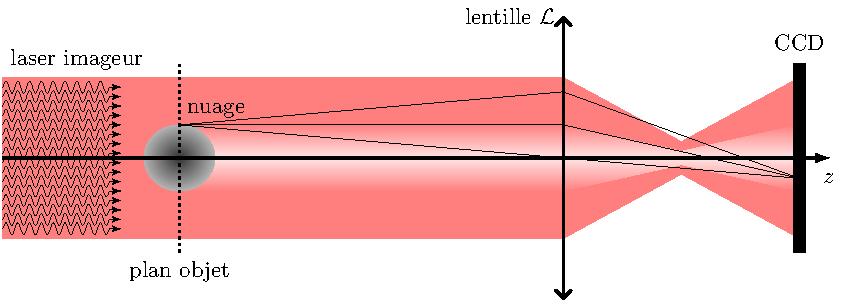
\includegraphics{P3/OptiqueAbsorption}
\CaptionFigss{Schéma illustrant un système optique simple pour faire une image par absorption. Le nuage absorbe une partie de la lumière laser incidente. L'image de cette ombre est recueillie par le capteur CCD.}
\label{fig:OptiqueAbsorption}
\efigh


Tout au long de sa propagation à travers le \n, le faisceau laser est absorbé, et diffusé. Nous considèrerons un faisceau laser se propageant selon la direction $z$. L'expression~\nref{eq:Pdif} permet de déterminer la variation élémentaire $\Diff{\Ilaser}$ d'intensité du laser lors de la propagation dans le nuage sur une longueur $\dz$:
\begin{align}
	\Diff{\Ixyz}
	& = \frac{\Diff{\Pdif}}{\dx\,\dy} 
	\nonumber\\
	& = \hbar\,\pulsReso\, \pulsSpont \, \frac{1}{2} 
	\, \frac{\sat}{1+\sat}
	\, \densxyz\,\dz 
	\pointformule
	\label{eq:dIabsGenerale}
\end{align}
En faisant apparaître explicitement la dépendance en intensité dans le paramètre de saturation~(expression~\nref{eq:ParamSat}), nous obtenons une équation différentielle non-linéaire du premier ordre vérifiée par $\Ixyz$ au cours de la traversée du nuage:
\begin{align}
	\Derive{\Ixyz}{z}
	& = - \frac{\hbar\,\pulsReso\, \pulsSpont}{2} 
	\, \IsurIsatxyz 
	\, \frac{1}{1 + \IsurIsatxyz + \left(\dfrac{2\,\desac}{\pulsSpont}\right)^2}
	\, \densxyz 
	\pointformule
	\label{eq:EqDiffAbsGenerale}
\end{align}

\subsubsection{Absorption dans le régime de saturation faible}
La technique usuelle d'imagerie par absorption consiste à utiliser un faisceau laser résonant ($\desac=0$), et dont l'intensité est faible devant \lintsat. On parlera alors d'\emph{imagerie par absorption dans le régime de saturation faible.} Dans cette limite, on peut considérer que les atomes ont une réponse linéaire à l'intensité laser.
L'expression~\nref{eq:dIabsGenerale}, avec $\sat\ll 1$ permet ainsi d'obtenir l'équation différentielle linéaire du premier ordre :
\begin{align}
	\Derive{\Ixyz}{z}
	& =
	- \seceff
	\, \Ixyz
	\, \densxyz
	\virguleformule
	\label{eq:EqDiffAbsBasseInt}
\end{align}
où $\seceff = \frac{\hbar\,\pulsReso\, \pulsSpont}{2\,\Isat}$ %
\nome{\seceff}{Section efficace à résonance de la transition}%
est la \seff \emph{à résonance} de la transition excitée par le laser. Pour un système à deux niveaux, et d'après l'expression~\nref{eq:IsatExpr}, elle s'exprime très simplement en fonction de la \lo $\lambda$ du laser :
\[
\seceff = \frac{3\,\lambda^2}{2\,\pi}
\pointformule
\]
%\RemarqueTitre{Section efficace d'une transition}{La \seff $\seceff$ correspond à une surface imaginaire qui permet de rendre compte de la probabilité qu'un photon soit absorbé par l'atome.}
%
L'équation différentielle~\nref{eq:EqDiffAbsBasseInt} est remarquablement simple et se résout exactement :
\Resultat{ 
Si nous désignons par $\Iinxy$ l'intensité du laser lorsque celui-ci atteint le nuage, nous pouvons exprimer l'intensité $\Ioutxy$ du laser après la traversée du \n par la relation:
\begin{equation}
\Ioutxy = \Iinxy \, \expo{-\seceff\,\denscolxy}
\virguleformule	
	\label{eq:BeerLambert}
\end{equation}
qui n'est rien d'autre que la loi de Beer-Lambert, \cad la loi régissant l'absorption dans un milieu ayant une réponse \emph{linéaire} à l'intensité. La quantité sans dimension $\seceff\,\denscolxy$ est appelée \emph{\pro} et pourra être notée $\OptProf\xy$.
}%
\nomeRemonte{\Iin}{Intensité incidente du laser imageur sur le \n}{4cm}%
%
\nomeRemonte{\Iout}{Intensité du laser imageur après la traversée du \n}{3cm}%


\casse
%
\noindent
Pour la suite de ce chapitre, il sera utile de différentier les deux quantités physiques suivantes:
\begin{itemizel}
	\item la \emph{\pro} %
\nome{\OptProf}{Profondeur optique du \n selon l'axe $z$}%
:
\begin{equation}
	\OptProf\xy \equiv \seceff\,\denscolxy
	\label{eq:DefOptProf}
	\virguleformule
\end{equation}
	qui est une \emph{caractéristique propre} du \nat, et dont la valeur est par définition indépendante de la méthode employée pour la mesure,
	\item et la \emph{\do} que nous définissons par %
\nome{\OptDens}{Densité optique du \n selon l'axe $z$}%
:
\begin{equation}
	\OptDens\xy 
	\equiv \Ln{	\frac{\Iinxy}{\Ioutxy}	}
	\virguleformule
\end{equation}
%$\vspace{-6pt}
et qui décrit l'\emph{atténuation relative de la lumière} laser traversant le \n. 
\end{itemizel}
\Resultat{
Dans le protocole d'\ipafas ces deux grandeurs sont égales : $\OptProf=\OptDens$. Dans les~\autoref{sec:LimitesNuageDense} et~\nref{sec:ipafos} nous seront amenés à considérer le fait que $\OptProf$ et $\OptDens$ ne sont pas égales en général. La \do dépend, entre autres choses, de l'intensité et du désaccord du laser imageur.
}



\subsubsection{Protocole de mesure}
En pratique, comme dans le cas de l'imagerie par fluorescence, le capteur CCD mesure une lumière de fond $\Ibackxy$. Le protocole d'extraction de la \dcol $\denscolxy$ consiste à capturer trois images:
\begin{itemize}
	\item la première est une image du \nat, en présence de la lumière laser excitatrice; le signal recueilli correspond à $\Iccdxy = \Ibackxy + \Ioutxy$.
	\item la deuxième est une image prise dans les mêmes conditions, \emph{mais en l'absence du nuage}; le signal mesuré est alors $\Iccdxy = \Ibackxy + \Iinxy$ puisque le laser n'est pas absorbé.
	\item la troisième est une image prise dans les mêmes conditions, \emph{mais en l'absence du nuage et du laser imageur}; le signal mesuré est alors composé uniquement du terme $\Ibackxy$.
\end{itemize}
\Resultat{
Une opération mathématique effectuée pour chaque pixel $\xy$ du capteur CCD permet alors de calculer la \dcol:
\begin{align}
	\seceff \, \denscolxy 
	& = 
	\Ln{
	\frac{
	\IccdxySansNuage - \Ibackxy
	}{
	\IccdxyAvecNuage - \Ibackxy
	}
	} \nonumber \\
	& = 
	\Ln{
	\frac{\Iinxy}{\Ioutxy}
	}
	\equiv \OptDens\xy
	\label{eq:DensColAbsorption}
\end{align}
\ff
}
Ce protocole d'imagerie par absorption dans le régime de \emph{saturation faible} possède une qualité majeure : la sensibilité du capteur CCD, ainsi que les caractéristiques de la transition ($\Isat$, $\seceff$) n'ont pas besoin d'être connues pour donner des mesures quantitatives
\footnotemark
 de \do. En effet, seul le rapport des deux intensités $\Iin$ et $\Iout$ intervient. 
%En revanche, il est nécessaire de connaître avec précision la \seff $\seceff$ de la transition pour pouvoir calculer la \dcol. 
%Ce point apparemment anodin sera abordé dans la~\autoref{sec:ipafos}.
\footnotetext{Attention cependant: en ce qui concerne la \pro, nous montrerons dans la suite que l'interprétation d'images par absorption peut être erronée si la \seff \emph{effective} (voir la~\autoref{sec:ipafos}) n'est pas précisément mesurée.}

\casse

\noindent
La figure~\nref{fig:ImagesAbsor} représente un exemple d'images prises pour le protocole d'imagerie par absorption.
\bfighss
\subfloat[sans \n]{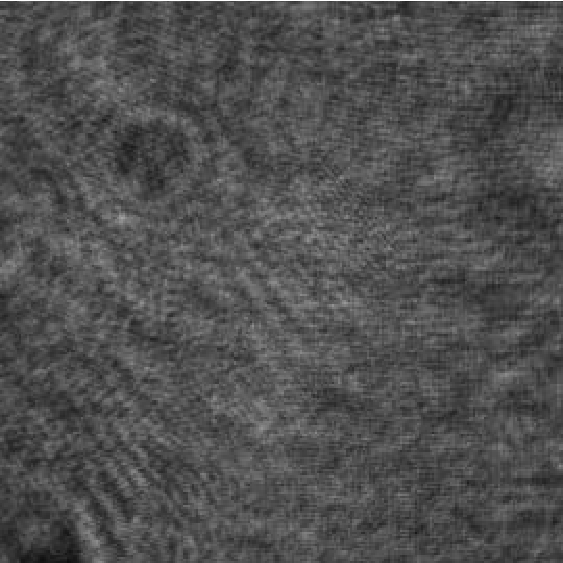
\includegraphics[width=4.5cm]{P3/2005_12_16_A_movie_2_00060_NoAt}}\,
\subfloat[avec \n]{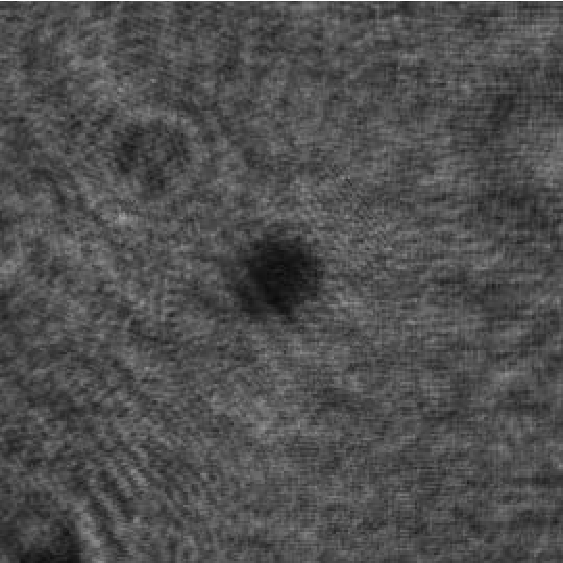
\includegraphics[width=4.5cm]{P3/2005_12_16_A_movie_2_00060_With}}\,
\subfloat[\dcol]{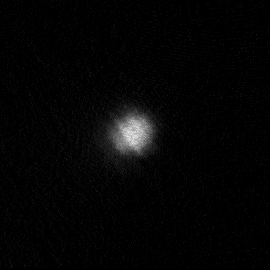
\includegraphics[width=4.5cm]{P3/2005_12_16_A_movie_2_00060Absor}}
\CaptionFigs{Exemple d'images prises pour le protocole d'imagerie par absorption. L'image (a) correspond à la lumière laser seule, \cad en l'absence du \nat. L'image (b) est prise dans les mêmes condion que l'image (a), mais en présence du \n. L'image \sotosay{de fond} n'est pas représentée car elle est essentiellement toute noire. En appliquant la formule~\nref{eq:DensColAbsorption} à chaque pixel $\xy$, on obtient l'image (c) qui représente la \do $\OptDens\xy$ du nuage.}
\label{fig:ImagesAbsor}
\efigh


\section{Fiabilité d'une mesure sur un \n très dense}\label{sec:LimitesNuageDense}
Les deux techniques précédemment décrites dans la~\autoref{sec:ImagerieUsuelles} sont assez simples à mettre en \oe uvre et sont largement utilisées. Cependant, nous allons voir, dans cette section, que le traitement de nuages très denses rend ces techniques peu adaptées~\cite{KDS99,KSN01}. Nous allons ici souligner les limites de ces protocoles.%, puis nous évoquerons succinctement deux exemples de techniques développées dans d'autres groupe pour obtenir des images exploitables de \nats denses.


\subsection{Limites du protocole d'\ipf}
Lors de l'étude théorique du protocole d'\ipf~(\autoref{sec:ipf}), nous avons implicitement fait une hypothèse simplificatrice importante. Celle-ci consiste à considérer que tous les photons émis spontanément au sein du nuage peuvent atteindre le capteur CCD avec la même probabilité. 
%
En réalité, il se peut qu'un photon diffusé par un atome soit immédiatement ré-absorbé dans le \n par un autre atome.
\inlinefig{\includegraphics{P3/EmissionRéabsorption}}
\noindent En quoi ce phénomène est-il gênant?

\noindent Si les photons émis au sein du nuage ont une probabilité non-négligeable d'y être ré-absorbés, alors le système optique (lentille + capteur CCD) ne \sotosay{percevra} pas de la même manière tous les atomes, selon leurs positions dans le nuage. L'illustration ci-contre représente les trajets de deux photons émis par deux atomes, pris arbitrairement de part et d'autre du nuage. L'un des deux photons (celui de gauche) aurait dû être collecté par le système optique, mais ne le sera pas à cause des ré-absorptions successives.
Ceci revient à dire que le système optique ne peut observer que la surface apparente du \n.
\picskip{0}
\noindent Pour dégager un critère de fiabilité, il faut considérer le \termetech{libre parcours moyen} $\Dlibre$ %
\nome{\Dlibre}{Libre parcours moyen d'un photon dans le \n}%
d'un photon dans le \n. Dans un nuage de \dat typique $\overline{\dens}$, le libre parcours moyen $\Dlibre$ est défini par:
\begin{equation}
	\Dlibre \, \seceffsat \, \overline{\dens} \equiv 1
	\virguleformule
	\label{eq:LibreParcours}
\end{equation}
où $\seceffsat$ est la \seff de la transition en tenant compte de la saturation:\label{sec:ReAbsorption}
\begin{equation}
	\seceffsat \equiv \seceff \, \frac{1}{1+\sat}
	\pointformule
	\label{eq:SecEffSat}
\end{equation}
%
\noindent
On peut dégager deux comportements limites en fonction de la taille caractéristique $\LZnuage$ du \n suivant l'axe optique: 
\begin{itemize}
	\item si $\Dlibre\gg\LZnuage$, alors un photon aura peu de chance d'être ré-absorbé dans le \n, 
	\item en revanche, si $\Dlibre \ll \LZnuage$, chaque photon diffusé sera très probablement ré-absorbé, puis ré-émis, puis ré-absorbé,... un grand nombre de fois avant de quitter le \n.
\end{itemize}
%
\Resultat{
En considérant que la \dcol $\denscol$ du \n est de l'ordre de $\overline{\dens} \, \LZnuage$, et d'après les expressions~\nref{eq:SecEffSat} et~\nref{eq:LibreParcours}, nous pouvons dégager un critère sur la \pro du nuage.
Ainsi, les processus de ré-absorption peuvent être négligés si
\begin{equation}
	\seceff \, \denscol \ll  1+\sat
	\pointformule
	\label{eq:NegligeReAbsorption}
\end{equation}
\finformule
}
\ApplicationNumerique
{\label{an:ProfondeurOptiques}
Estimons l'intensité nécessaire pour obtenir une image exploitable dans deux cas usuels:
\begin{ditemize}
	\item dans le \pmo décrit dans la~\autoref{sec:PaquetsPmo},  la \dat d'un nuage est typiquement \atpcc{2E{10}}. Avec une taille transverse (suivant l'axe du système optique) $\LZnuage\approx\mm{5}$, la \pro atteint  
\[
\AvecTexte{\seceff \, \denscol}{\tiny PMO} \approx 30
\pointformule
\]
\item dans un \bec de \rb, la \dat atteint typiquement \atpcc{E{14}}. Considérons une taille typique $\LZnuage\approx\micron{10}$. Dans ces conditions la \pro atteint  
\[
\AvecTexte{\seceff \, \denscol}{\tiny BEC} \approx 300
\pointformule
\]
\end{ditemize}
On constate donc qu'il faut disposer d'intensités très importantes. En effet l'expression~\nref{eq:NegligeReAbsorption} qui donne le critère de validité d'une mesure, impose l'utilisation d'intensités des centaines voire des milliers de fois supérieures à \lintsat.
}

\casse 

\subsubsection{\Ipf dans un régime extrêmement saturant}
L'équipe de D.~Weiss (Berkeley, Californie) a mis en \oe uvre un protocole d'\ipf dans un régime de saturation extrême  afin d'étudier un \pmo comprimé d'atomes de Césium~\cite{DLH00}. Il utilise un laser Titane-Saphir délivrant \SI{500}{\milli\watt} de lumière résonante. Le laser imageur est rétro-réfléchi de manière à équilibrer les forces radiatives induites par l'absorption répétée de photons. Avec un faisceau imageur dont le rayon à $\ttfrac{1}{\expo{2}}$ de \mm{4}, il est possible d'obtenir des intensités allant jusqu'à $\val{2000} \, \Isat$. 

\noindent
Le fait d'utiliser de telles intensités est très intéressant à plusieurs égards sur le plan physique :
\begin{ditemize}
	\item la population $\PopuE$ de l'état excité est très proche%
	\footnote{On peut montrer que dans la limite $\sat\gg1$ la différence de population entre état excité et état fondamental est $\PopuE - \PopuG \approx-\ttfrac{1}{\sat}$.} 
	de sa valeur limite $\PopuEmax=\tfrac{1}{2}$. Ainsi, \emph{chaque atome} émet en moyenne $\tfrac{\pulsSpont}{2}$ photons par seconde, indépendamment \emph{des fluctuations locales d'intensité} dans le faisceau laser. Les mesures sont donc quantitatives.
	\item le paramètre de saturation $\sat$ est grand devant l'unité, et ce, même si le laser n'est pas parfaitement à résonance. Cette méthode est ainsi insensible au désaccord du laser ou à la présence de \gchm. Elle est en particulier utilisable pour effectuer une image d'un \pmo.
	\item la section efficace $\seceffsat$ de la transition saturée est très faible (voir \vpageref{sec:ReAbsorption}). Ainsi, les \dos mesurables sont beaucoup plus élevées. Une autre interprétation physique de ce phénomène est que les processus de ré-absorption au sein du \n sont compensés par les processus d'émission stimulée, puisque la population $\PopuE$ de l'état excité est presque identique à la population $\PopuG$ de l'état fondamental.
\end{ditemize}
La technique décrite dans la référence~\cite{DLH00} est donc précise, robuste et a permis au groupe de D.~Weiss de mesurer des \do de l'ordre de \val{100}.

%Ce protocole n'est cependant pas de toute simplicité à mette en \oe uvre, tant du point de vue matériel (un laser Titane-Saphir coûte typiquement cent milles euros), que du point de vue technique (un alignement soigneux du laser rétro-réfléchi est primordiale).

\subsection{Limites de l'\ipafas}\label{sec:LimiteIpafas}
Lors d'une capture d'image, les données sont enregistrées, puis traitées par un système informatique. Ceci implique une numérisation des signaux fournis par le capteur CCD. 
Dans cette sous-section nous montrons en quoi cela interdit de mesurer des \dos élevées par la technique d'\ipafas. 


\subsubsection{Numérisation du signal fourni par le capteur CCD}\label{sec:SignalCCD}
	Le signal $\Signal\xy$ que le capteur CCD délivre est le résultat d'une conversion analogique-numérique sur un nombre $\Nbit$ de bits. Ceci implique une \emph{discrétisation de l'amplitude} du signal $\Signal\xy$ puisqu'il ne peut prendre que $2^{\Nbit}$ valeurs possibles:%. Par exemple, si $\Nbit=8$ seul \val{256} valeurs:
\[
000...01,~~000...10,~~000...11,\ldots\ldots\ldots,~~111...10~\text{et}~~111...11
\pointformule
\] 
%
\noindent En pratique, en utilisant un gain électronique ou en jouant sur le temps d'exposition du capteur, on peut ajuster la valeur maximale $\SignalMax$ que l'on peut mesurer, \cad la valeur de $\Signal$ qui correspond au nombre binaire $111...11$. Le \emph{pas de discrétisation} $\SignalPas$, \cad la valeur de $\Signal$ qui correspond au nombre binaire~$000...01$, est alors donné par la relation: 
	\[
	\SignalPas = \frac{\SignalMax}{2^{\Nbit}-1} % \approx \frac{\SignalMax}{2^{\Nbit}}
	\virguleformule
	\]
où $\SignalPas$ est la limite de précision sur le signal fournit par le capteur.
\Remarque{
Il faudrait en fait aussi tenir compte du bruit électronique de la caméra. Celui-ci joue un rôle important dans l'interprétation des signaux. Notons cependant que, même en l'absence totale de bruit, la discrétisation de l'amplitude reste la limite ultime de précision. Nous négligerons dans la suite les effets du bruit pour nous concentrer sur l'effet de la numérisation.
}

\ApplicationNumerique
{
Le capteur CCD utilisé sur notre \setup est un modèle \textbf{Basler A102 f} monochrome. %dont la fenêtre de protection a été retirée afin d'éviter des phénomènes d'interférences par réflexions multiples.
%La taille des pixels est de $\micron{6.45} \times \micron{6.45}$. 
Le signal est numérisé sur $\Nbit=8$ ou $12$ bits au choix. La sensibilité du capteur a été calibrée par nos soins. 
 Pour la longueur d'onde que nous utilisons ($\nm{780}$) et en l'absence de gain électronique, le pas de discrétisation ainsi mesuré correspond à une énergie de~$\SI{9.3E-17}{\joule}$, soit $365$ photons.
}

\subsubsection{Limites de \do mesurable avec l'\ipa}

Soulignons maintenant les limites du protocole d'\ipafas décrit dans la~\autoref{sec:ipafas}. 
L'exploitation des images prises par cette méthode se fait grâce à l'expression~\nref{eq:DensColAbsorption} que nous rappelons ici:
\[
	\seceff \, \denscolxy 
	= 
	\Ln{
	\frac{\Iinxy}{\Ioutxy}
	}
	\equiv \OptDens\xy
	\text{~~~~(rappel de l'équation~\nref{eq:DensColAbsorption} page  \pageref{eq:DensColAbsorption})}
\pointformule
\]
Or, si la \do du nuage est importante, alors la valeur de l'intensité $\Iout$ après la traversée du nuage peut devenir extrêmement faible%
%
\footnote{Par exemple, une \do de \val{7} revient à diviser l'intensité par un facteur $\expo{-7}\approx\val{1000}$ lors de la traversée du nuage.}
%
 par rapport à l'intensité incidente $\Iin$. En d'autres termes, le nuage peut absorber la quasi-totalité de la lumière incidente.

Nous allons montrer que ceci pose un réel problème de mesure avec le capteur CCD. 
%En effet, comme nous l'avons mentionné dans la~\autoref{sec:SignalCCD}, le signal $\Signal\xy$ fourni par le capteur CCD est quantifié, et ne peut prendre que $2^\Nbit$ valeurs possibles comprises entre $0$ et $\SignalMax$. Le pas de discrétisation $\SignalPas$ est déterminé par le nombre $\Nbit$ de bits de codage. Il est important d'utiliser au mieux toute la plage des valeurs possibles pour l'acquisition d'images. 
Afin d'utiliser au mieux toute la plage des valeurs possibles pour le signal $\Signal\xy$,
%Pour ce faire, 
nous réglons le système optique de manière à ce que la valeur $\SignalMax$ corresponde à l'intensité maximale du laser imageur quand celui-ci n'est pas absorbé, \cad:
\[
\SignalMax \, \longleftrightarrow \, \Iinmax \equiv \sup(\Iinxy)
\pointformule
\] 
%Toute intensité supérieure à $\Iinmax$ serait mesuré par le capteur.
Le pas de discrétisation $\SignalPas$ correspond alors à :
\[
\SignalPas = \frac{\SignalMax}{2^\Nbit-1} 
\quad \longleftrightarrow \quad 
\IPas = \frac{\Iinmax}{2^\Nbit-1}
\pointformule
\]
Ceci impose une discrétisation des valeurs obtenues grâce à l'expression~\nref{eq:DensColAbsorption} qui fait intervenir le rapport des deux intensités $\Iin$ et $\Iout$. 
Il est en particulier important de s'interroger sur la précision obtenue lorsqu'on utilise cette expression avec $\Iin$ et $\Iout$ prenant des valeurs discrètes par pas de $\IPas$. Une simple différentiation de l'expression~\nref{eq:DensColAbsorption} nous permet d'estimer la précision de la mesure:
\begin{align}
\Delta \left( \seceff \, \denscol \right) & = \frac{\IPas}{\Iout}+\frac{\IPas}{\Iin} \nonumber \\
& \approx \frac{\IPas}{\Iout} \qquad \text{puisqu'on suppose que $\Iout\ll\Iin$} \nonumber
\pointformule
\end{align}
 
\ApplicationNumerique{
Estimons les \dos maximales auxquelles nous pouvons avoir accès, en tenant compte de la discrétisation du signal provenant du capteur CCD, dans les deux cas suivants:
\begin{itemize}
	\item pour un codage sur $\Nbit=8$ bits, l'expression~\nref{eq:DensColAbsorption} peut donner une valeur qui vaut au plus
\[
	\OptDens
	=  
	\Ln{
	\frac{\SignalMax}{\SignalPas} 
	}
	= 
	\Ln{ 2^\Nbit-1 } 
	\approx \val{5.5}
	\pointformule
\]
Cependant, si nous voulons disposer d'une précision relative de $10\%$, la \do calculée ne doit pas excéder $\OptDens=\val{4.5}$.
\item dans le cas $\Nbit=12$, la \do calculée vaut au plus $\OptDens=\val{8.3}$, mais pour pouvoir disposer d'une précision relative de $10\%$, la \do devra être inférieures à $\OptDens=\val{7.5}$ 
\end{itemize}
}
Nous comprenons donc pourquoi le protocole d'\ipafas est limité à des mesures de \pro de l'ordre de \val{4}-\val{5}.
Nous montrerons dans la~\autoref{sec:ipafos} comment ce problème peut être contourné en utilisant la réponse non-linéaire des atomes.

\subsection{Absorption d'un faisceau laser désaccordé}\label{sec:ImagerieDesaccordee}
Une manière de contourner cette limite est de diminuer l'absorption du laser imageur en jouant sur le désaccord $\desac$ du laser. En effet, l'expression \vref{eq:Pdif} montre que l'on peut réduire l'absorption en désaccordant le laser imageur. On montre alors que l'expression~\nref{eq:DensColAbsorption} devient :
\begin{equation}
	\OptDens\xy 
	\equiv 	\Ln{	\frac{\Iinxy}{\Ioutxy}	}
	= \frac{\seceff\,\denscolxy}{1+\left(\dfrac{2\,\desac}{\pulsSpont}\right)^2} 
\virguleformule
	\label{eq:ODhorsReso}
\end{equation}

\ApplicationNumerique{
Il suffit par exemple de régler le désaccord à $\delta=\pulsSpont$ pour qu'une \do de $7$ à résonance devienne proche de l'unité. 
}
Cependant, pour un laser non-résonant, le nuage atomique se présente comme un milieu dispersif. Pour un atome à deux niveaux, l'indice de réfraction $\nrefracImaginaire$ est donné par~\cite{KDS99}:
\[
	\nrefracImaginaire\xyz 
= 1 + \dens\xyz \, \frac{\seceff\,\lambda}{4\,\pi} 
\, \left(
\frac{ \im }{1+\left(\dfrac{2\,\desac}{\pulsSpont}\right)^2}
-
\frac{ \dfrac{2\,\desac}{\pulsSpont} }{1+\left(\dfrac{2\,\desac}{\pulsSpont}\right)^2}
\right)
\virguleformule
\]
%
où $\lambda$ est la longueur d'onde du laser, et $\dens\xyz$ est la \dat du nuage. La partie imaginaire de $\nrefracImaginaire$ correspond au caractère absorbant du milieu. La partie réelle de $\nrefracImaginaire$ :
\begin{equation}
	{\nrefracxyz}
= 1 - \dens\xyz \, \frac{\seceff\,\lambda}{4\,\pi} 
\, \frac{ \dfrac{2\,\desac}{\pulsSpont} }{1+\left(\dfrac{2\,\desac}{\pulsSpont}\right)^2}
\virguleformule
	\label{eq:nrefraction}
\end{equation}
correspond au caractère dispersif qui induit le déphasage de l'onde et par suite sa réfraction.
 

\casse
 
\inlinefig{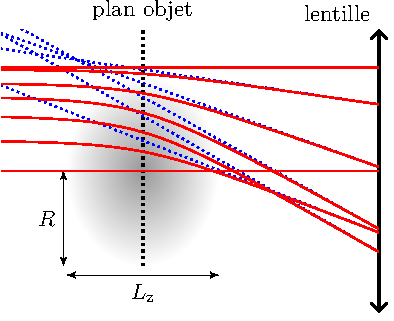
\includegraphics{P3/LentilleGradientIndice}}%
Ce phénomène de réfraction fait que l'ensemble atomique agit comme une lentille à gradient d'indice sur le faisceau laser imageur. Les rayons lumineux sont déviés, si bien que l'image obtenue sur le capteur CCD, qui correspond à l'intensité lumineuse provenant du plan objet, sera déformée : c'est un effet de \sotosay{mirage optique}. Sur l'illustration ci-contre, nous représentons quelques rayons lumineux, ainsi que leurs prolongations (en pointillé) dans le plan objet. La déviation des rayons vers le centre du nuage (où la \dat est élevée) traduit le fait que ${\nrefrac}$ est ici supérieur%
\footnote{Le laser imageur doit être dans ce cas désaccordé sur le rouge de la transition ($\desac < 0$).}
à \val{1}.
%\picskip{0}

La figure~\nref{fig:ImageNuageDesaccorde} donne un exemple d'images effectuées sur un \nat dense, avec un désaccord nul, puis avec un désaccord $\desac=-2\,\pulsSpont$.
On y constate clairement l'effet de lentille sur la deuxième image.
\bfighss
\subfloat[$\desac = 0$]
{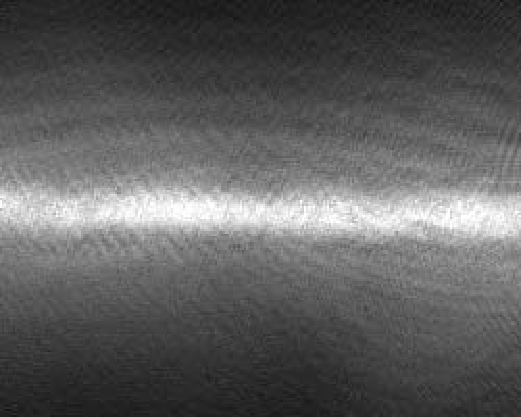
\includegraphics[width=6cm]{P3/Det0Gamma_000Absor}}\qquad
\subfloat[$\desac=-2\,\pulsSpont$]
{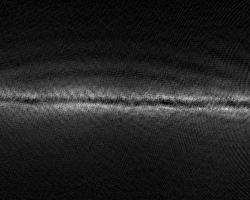
\includegraphics[width=6cm]{P3/Det+2Gamma_000Absor}}
\CaptionFigs{Exemples d'images effectuées sur un \nat dense produit par un \pmobd comprimé (du fait de la forme longiligne du \n, on n'en distingue qu'une partie sur ces images). 
L'image (a) est prise par la technique d'\ipafas décrite dans la~\autoref{sec:ipafas}, avec un laser résonant ($\desac=0$). 
L'image (b) est prise dans les mêmes conditions expérimentales, mais en désaccordant le laser imageur de $\desac=-2\,\pulsSpont$.
On observe clairement l'effet de lentille sur la deuxième image : la zone centrale y est sombre du fait de la réfraction des rayons du faisceau imageur.
}
\label{fig:ImageNuageDesaccorde}
\efigh


Dégageons un critère qui permette de déterminer si l'image d'un nuage avec un faisceau désaccordé sera exploitable.
\newline
\noindent La réfraction du faisceau laser rend en pratique l'image quasiment inexploitable si, lors de la traversée du nuage, les rayons lumineux sont déviés transversalement (dans le plan objet) d'une distance non négligeable devant la taille transverse du nuage $2\,\Rnuage$.
%
L'équation qui décrit la propagation des rayons lumineux dans le nuage est tirée de l'équation \termetech{iconale} et peut se mettre sous la forme :
\[
%\DepartHighlightColorMath{blue}
{
\Derive{}{s}\left(~\nrefrac\,\Vecteur{u} \right)}
 = 
%\DepartHighlightColorMath{red}
{\Gradient{\nrefrac}}
\virguleformule
\]
où $\Vecteur{u}$ est le vecteur unitaire porté par la trajectoire du rayon lumineux et $s$ est l'abscisse curviligne le long de la trajectoire.
Un calcul d'ordre de grandeur permet d'estimer la déviation typique $\deviR$ d'un rayon dans le plan transverse après la propagation au travers du nuage sur une longueur $\LZnuage$ :
\[
%\ArriveeHiglightColorMath{blue}
{
~\nrefrac\,\frac{\deviR}{\LZnuage^2} \approx \frac{\deviR}{\LZnuage^2} }
 \approx 
% \ArriveeHiglightColorMath{red}
 {\frac{\nrefrac-1}{\Rnuage}}
 \pointformule
\]%
%\MakeFlecheHighlightColor{blue}
%\MakeFlecheHighlightColor{red}
%
\Resultat{
En utilisant les expressions~\nref{eq:ODhorsReso} et~\nref{eq:nrefraction} nous pouvons extraire le critère suivant qui permet d'estimer que l'effet de la réfraction est négligeable:
\[
\frac{\deviR}{\Rnuage} \approx 
\OptDens%\frac{\seceff\,\denscol}{1+\left(\dfrac{2\,\desac}{\pulsSpont}\right)^2}
\,\frac{\lambda\,\LZnuage}{\Rnuage^2} 
\, \frac{\desac}{\pulsSpont}
\ll 1
\virguleformule
\]
Cette expression fait intervenir la \do hors résonance, qui rappelons le, doit être de l'ordre de l'unité afin d'obtenir une image de qualité. 
}
\ApplicationNumerique
{
Calculons ce critère dans les deux cas usuels considérés précédemment (page \pageref{an:ProfondeurOptiques}):
\begin{ditemize}
	\item la \pro $\OptProfExpr \approx 30$ d'un nuage du \pmo, nous incite à utiliser un désaccord $\desac \approx 1.5\,\pulsSpont$. Le \n ayant une taille typique \mbox{$\LZnuage\approx2\,\Rnuage\approx\mm{5}$}, nous obtenons:
\[
\AvecTexte{\frac{\deviR}{\Rnuage}}{\tiny PMO} \approx ~~ \frac{\lambda\,\LZnuage}{\Rnuage^2} 
\, \frac{\desac}{\pulsSpont} 
~~ \approx ~~ \val{3E{-3}}
\pointformule
\]
\item dans un \bec d'atome de \Rb, la \pro est typiquement $\OptProfExpr \approx 300$ et les dimensions \mbox{$\LZnuage\approx2\,\Rnuage\approx\micron{10}$}. En utilisant un désaccord de $\desac \approx 5\,\pulsSpont$, nous obtenons:
\[
\AvecTexte{\frac{\deviR}{\Rnuage}}{\tiny BEC} \approx ~~  \frac{\lambda\,\LZnuage}{\Rnuage^2} 
\, \frac{\desac}{\pulsSpont} 
~~ \approx ~~ \val{5}
\pointformule
\]
\end{ditemize}
On peut donc a priori utiliser un laser désaccordé dans le premier cas, mais pas dans le second.
}

%
\RemarqueTitre{Imagerie par contraste de phase}{
Une technique d'imagerie dite \termetech{par contraste de phase}~\cite{KDS99} consiste précisément à exploiter le déphasage de l'onde laser par le \n afin de mesurer la partie réelle de l'indice de réfraction par une méthode interférométrique. 
%Le capteur CCD fait alors l'image de la distribution d'intensité dans un plan objet situé en aval du nuage. 
%Un algorithme mathématique permet d'obtenir la \dcol du nuage. 
Une démonstration expérimentale de cette méthode très efficace fait l'objet de la référence~\cite{TWP04}.
}
%i)Exemple gradient indice gaussien : que voit la caméra en fonction du désaccord
%1 page sur phase contraste imaging --> Livre Varenna 1999 (p97) (indice p95)\cite{TWP04}


\casse


\subsection{Absorption sur une transition ouverte}\label{sec:ImagerieFun}

Une autre méthode pouvant être utilisée pour obtenir une image par absorption d'un nuage optiquement épais consiste à utiliser le laser imageur non pas sur la transition cyclante%
% $\TransGE$
, mais sur une \emph{transition ouverte}%
\footnote{Nous avons précédemment mentionné cette technique dans la section \vref{sec:MesureDensiteGuide}.}%
. 
%Sur une transition ouverte, chaque atome ne peut absorber qu'un nombre fini de photons, si bien que le \nat ne  

\subsubsection{Deux photons pour chaque atome}
\noindent Dans le cas de l'atome de \Rb, nous utilisions la transition $\TransOpen$.
Quand un atome est excité sur cette transition ouverte%
\footnote{Cette transition est habituellement utilisée pour \termetech{repomper} les atomes dans l'état \EtatSF{2} à l'intérieur d'un \pmo.}%
, il y a alors une probabilité 
\[
p = \frac{1}{2}
%\virguleformule
\]
pour que celui-ci retombe dans l'état \EtatSF{1}, devenant une nouvelle fois candidat à l'absorption d'un photon. Si l'atome retombe%
\footnote{La probabilité de retomber dans $\EtatSF{2}$ est naturellement égale à $1-p= \frac{1}{2}$.}
 dans \EtatSF{2}, il ne pourra plus absorber les photons du laser. 

De manière à rendre une telle mesure d'absorption quantitative, nous devons calculer le nombre de photons qui seront absorbés par chaque atome, en moyenne. La probabilité $P(n)$ qu'a un atome d'absorber exactement $n$ photons correspond à la probabilité de retomber $n-1$ fois dans \EtatSF{1}, puis, de tomber dans \EtatSF{2}:
\[
P(n) = p^{n-1}\,(1-p)
\pointformule
\]
\Resultat
{
Nous déduisons donc le nombre moyen $\Moyenne{n}$ de photons absorbés par un atome avant qu'il ne tombe dans l'état \EtatSF{2}:
\[
\Moyenne{n} 
= \sum_{n=1}^{\infty} n\,P(n) 
= \sum_{n=1}^{\infty} n\,p^{n-1}\,(1-p) 
= \frac{1}{1-p} 
= 2
\pointformule
\]
Chaque atome absorbe donc en moyenne $2$ photons.
}	


\subsubsection{Intérêts et inconvénients}
\noindent
Cette technique d'imagerie sur une transition ouverte présente deux avantages majeurs:
\begin{itemizel}
	\item elle est quantitative dans la mesure où le nombre de photons absorbés reflète exactement le nombre d'atomes du nuage%
\footnote{Chaque atome absorbera 2 photons, mais à une condition, celle d'envoyer assez de lumière pour que tous les atomes tombent dans l'état \EtatSF{2}. Ceci ne pose en pratique aucune contrainte technique.}%
.
	\item elle est de plus d'une grande robustesse. En effet, la présence de \gchm, ou de toute autre source d'élargissement de la transition cyclante, ne modifie en aucun cas le caractère quantitatif de cette technique. 
\end{itemizel}

\casse

\noindent
L'inconvénient principal de cette méthode réside dans la faiblesse des signaux à mesurer, puisque le nombre de photons absorbés par unité de surface du faisceau imageur est de seulement deux fois la \dcol du \n.
\ApplicationNumerique{
Considérons un exemple pratique afin de montrer que le signal d'absorption sur une transition ouverte est très faible. Un nuage de typiquement \val{E9} atomes pourra absorber \val{2E9} photons. Si on considère que sa taille transverse
est $2\,\Rnuage\approx\mm{10}$, l'absorption par unité de surface du faisceau imageur est typiquement :
\[
2\,\denscol%\,\hbar\,\pulsReso 
\approx \frac{\val{2E9}}{\Rnuage^2} %\,\hbar\,\pulsReso
%\approx \SI{2E-9}{\joule\per\square{\centi\meter}}
\approx \SI{E10}{photon\per\square{\centi\meter}}
\pointformule
\]
La surface représentée dans le plan objet par un pixel du capteur CCD étant typiquement de $\Lpix=\micron{5}$, celui-ci devra être sensible à des variations très inférieures à \val{2500} photons. Cette performance est atteignable avec des capteurs CCD refroidis. 
}
\Remarque{Notons que l'utilisation d'une transition ouverte a aussi été étudiée dans le cadre de l'\ipf. On pourra consulter la référence~\cite{MOR07}.}


\section{Imagerie par absorption dans le régime de forte saturation}\label{sec:ipafos}
Dans cette section, nous allons décrire le protocole d'\ipa que nous avons mis au point afin de pouvoir acquérir, puis exploiter de manière \emph{quantitative}, des images d'ensembles atomiques \emph{denses.} 
%Sur le plan matériel, cette technique se base sur le même \setup que celui nécessaire pour l'\ipafas. 
Nous commencerons par donner quelques arguments qui remettent en cause le caractère quantitatif de l'\ipafas décrite dans la~\autoref{sec:ipafas}. Celle-ci est en effet assez sensible aux imperfections expérimentales.

\subsection{Position du problème}
Précisons tout d'abord un point important quant au caractère quantitatif de l'\ipafas. Nous avons précisé qu'un avantage certain de cette méthode est que la sensibilité du capteur CCD, ainsi que les caractéristiques de la transition ($\Isat$ et $\seceff$) n'ont pas besoin d'être connues pour donner des mesures quantitatives de \do (voir l'expression \vref{eq:DensColAbsorption}). En revanche, il est nécessaire de connaître avec précision la \seff $\seceff$ de la transition pour pouvoir calculer la \dcol $\denscol\xy$, grandeur qui nous intéresse.

\noindent Or, si pour un système à deux niveaux la \seff $\seceff$ de la transition s'exprime simplement:
\begin{equation}
	\seceff = \frac{3\,\lambda^2}{2\,\pi}
\virguleformule
	\label{eq:seff}
\end{equation} 
il faut en pratique tenir compte de la structure énergétique de l'atome.

\casse

\inlinefig{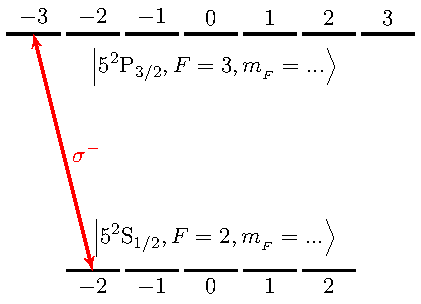
\includegraphics{P3/Rb2niveaux}}%
\noindent  
Ainsi, la sélectivité des règles de transitions entre \snx font que, dans le cas du \Rb, nous pouvons considérer la structure à deux niveaux $\{\EtatG$, $\EtatE\}$ décrite précédemment si, par exemple:
\begin{equation}
\begin{cases}
	\EtatG & = \EtatSFmF{2}{-2} \\
	\EtatE & = \EtatPFmF{3}{-3} 
\end{cases}
	\virguleformule
	\label{eq:Rb2niv}
\end{equation}
mais cela est valable \textbf{\emph{uniquement}} dans le cas où la lumière laser est \emph{parfaitement polarisée} circulairement $\sigma^{-}$. 
\picskip{1}

\noindent Si cela n'est pas le cas, les autres \snZs vont aussi se peupler et d'autre transitions vont intervenir. On ne peut alors théoriquement plus considérer l'expression~\nref{eq:seff} de la \seff comme valide%
%\footnote{Notons que la relation de proportionnalité \vref{eq:SectionEfficace} reste toujours valable.}%
.
De plus, d'autres imperfections expérimentales peuvent modifier le caractère absorbant du milieu atomique. On peut par exemple craindre : 
\begin{itemize}
%	\item la polarisation du laser n'est pas parfaite. Plusieurs \snZs sont alors occupés.
	\item que la pulsation du laser imageur ne soit pas exactement à la résonance ($\desac \neq 0$),
	\item que la largeur spectrale du laser soit non-négligeable devant la largeur naturelle $\pulsSpont$ de la transition,
	\item qu'un \chm résiduel déplace les \snZs, impliquant que le laser imageur devienne non-résonant.
\end{itemize}
	De plus, si l'impulsion laser est très courte, et que le nombre de photons absorbés par atome est de l'ordre de la dizaine, on doit considérer le régime transitoire des \EBO. La répartition initiale des populations des \snZs joue alors un rôle important dans l'absorption.

\Remarque{
Notons que l'effet des imperfections expérimentales est toujours de diminuer l'absorption de la lumière.
}

\noindent Existe-il un moyen d'extraire des informations quantitatives d'une image par absorption ?
Nous nous proposons dans la suite de ce chapitre de répondre à cette question. Nous décrirons les imperfections expérimentales par un \pdc, puis nous présenterons notre protocole d'imagerie qui permet de mesurer ce paramètre et d'interpréter quantitativement des images de \nats denses.

%Ceci a alors pour effet de diminuer la \seff d'interaction entre le laser et l'ensemble atomique. Parallèlement, \lintsat augmente%

\subsection{Intensité de saturation \emph{effective} et \seff \emph{effective}}

Dans toute la suite, nous désignerons par $\seceff$ et $\Isat$, la \seff et \lintsat de la transition fermée :
\[
\EtatSFmF{2}{-2}\longleftrightarrow\EtatPFmF{3}{-3}
\pointformule
\]
Il nous faut cependant rendre compte des inévitables imperfections expérimentales qui font que ce cas idéal de transition fermée n'est que théorique. 
%
\Resultat{
Nous supposerons qu'il est toujours possible de modéliser l'interaction des atomes du nuage avec l'onde laser par une \seff \emph{effective} $\seceffeff$ et une \intsat \emph{effective} $\Isateff$:
\begin{align}
	\seceffeff & \equiv \frac{\seceff}{\Imperf} \nonumber \\
	\Isateff & \equiv \Imperf\,\seceff 
	\virguleformule
	\label{eq:seffeffETintsateff}
\end{align}
où $\Imperf$ est un \pdc supérieur à $1$ qu'il faut déterminer expérimentalement. 
}%
\nomeRemonte{\seceffeff}{Section efficace effective}{3.3cm}%
%
\nomeRemonte{\Isateff}{Intensité de saturation effective}{2.4cm}%
%
\nomeRemonte{\Imperf}{Paramètre de correction rendant compte des imperfections expérimentales}{1.7cm}%

\noindent
L'équation~\nref{eq:DensColAbsorption} peut alors se réécrire sous la forme
\[
	\seceffeff \, \denscolxy = \frac{\seceff}{\Imperf} \, \denscolxy 
	= 	\Ln{	\frac{\Iinxy}{\Ioutxy}	}
\virguleformule
\]
qui permet de calculer $\denscolxy$ à partir de la connaissance de $\Iinxy$, $\Ioutxy$ et $\Imperf$.
Notons que $\Imperf$ est a priori spécifique à chaque situation expérimentale donnée, \cad qu'il doit être déterminé de manière systématique pour pouvoir exploiter des images prises par absorption.

~

Le problème est alors le suivant : 
\noindent comment déterminer $\Imperf$ sachant que ce paramètre n'intervient pas lors de la mesure de la \do et qu'on ne connaît a priori pas non plus la \dcol $\denscol\xy$ du nuage dont on fait l'image?\\
Nous allons montrer dans la suite que la réponse à cette question \ldots est non-linéaire.
%Nous allons montrer dans la suite que la réponse non-linéaire des atomes nous permet d'accéder à la valeur de $\Imperf$. 
%, tout en décrivant notre protocole d'imagerie adaptée aux nuages denses. 

\subsection{Réponse non-linéaire des atomes}
Nous avons vu dans la~\autoref{sec:LimiteIpafas} que la limite du protocole d'\ipafas réside dans le fait que la lumière laser peut être extrêmement atténuée lors de la traversée du nuage. Ce phénomène est principalement dû au caractère exponentiel de la loi de Beer-Lambert (voir l'équation différentielle linéaire \vref{eq:EqDiffAbsBasseInt}). 

On peut contourner cette limite en utilisant la réponse non-linéaire des atomes à une excitation laser, \cad en saturant la transition. Pour cela, nous utilisons des intensités laser plus élevées. On parle alors d'\emph{\ipadrfs}. 

Rappelons que, dans le cas général, l'évolution de l'intensité laser lors de la propagation dans le nuage est donnée par l'équation différentielle non-linéaire~\nref{eq:EqDiffAbsGenerale}. Celle-ci, dans le cas d'un laser résonnant ($\desac=0$), et en tenant compte du \pdc $\Imperf$, s'écrit:
\begin{equation}
	\Derive{\Ixyz}{z}
%	= - \densxyz
%	\, \seceffeff%\hbar\,\pulsReso\,\frac{\pulsSpont}{2} 
%	\, \frac{\Ixyz}{1 + \dfrac{\Ixyz}{\Isateff}}
	= - \densxyz
	\, \frac{\seceff}{\Imperf} 
	\, \frac{\Ixyz}{1 + \dfrac{\Ixyz}{\Imperf\,\Isat}}
	\pointformule
	\label{eq:EqDiffAbsResonance}
\end{equation}
%
Cette expression est valable pour toute valeur de l'intensité $\Ixyz$, à la différence de l'expression~\nref{eq:EqDiffAbsBasseInt}, qui n'est valide que dans la limite des faibles intensités .

\Resultat{
L'équation~\nref{eq:EqDiffAbsResonance} s'intègre par séparation de variables et permet de calculer la \dcol $\denscolxy$ à partir de la mesure de $\Iinxy$, $\Ioutxy$ et $\Imperf$, sans supposer que l'intensité est faible devant $\Isat$:
\begin{equation}
	\OptProfExpr\xy \equiv \OptProf\xyImperf 
	= \Imperf \, \Ln{	\frac{\Iinxy}{\Ioutxy}	}
	+ \frac{\Iinxy - \Ioutxy}{\Isat}
	\virguleformule
	\label{eq:DensColAbsHighIntResonance}
\end{equation}
où $\Iinxy$ et $\Ioutxy$ ont la même définition que dans la~\autoref{sec:ipafas}:
\begin{align}%\footnotesize
\begin{cases}
\Iinxy  \equiv & \IccdxySansNuage - \Ibackxy \nonumber 
\vspace{4pt} \\
\Ioutxy \equiv & \IccdxyAvecNuage - \Ibackxy \nonumber 
\end{cases}
%\pointformule
\end{align}
Notons que l'expression~\nref{eq:DensColAbsHighIntResonance}, prise dans la limite $\Iin,\Iout\ll\Isat$, redonne bien l'expression~\nref{eq:DensColAbsorption}, à une différence près cependant : le \pdc $\Imperf$ intervient dans le calcul de la \dcol.%
}
%
Nous devons souligner deux points importants relatifs à l'utilisation de l'expression~\nref{eq:DensColAbsHighIntResonance} afin d'exploiter l'\ipadrfs:
\begin{itemizel}
	\item il est indispensable de \emph{calibrer la sensibilité} du capteur CCD, afin de mesurer de manière absolue%
	\footnote{En effet, dans le cas de l'\ipafas de la~\autoref{sec:ipafas}, la sensibilité du capteur CCD n'avait pas besoin d'être calibrée, puisque seul  le rapport de deux intensités intervenait dans l'équation.}
	 la différence $\Iinxy - \Ioutxy$. Chaque pixel du capteur CCD fait alors office de puissance-mètre. Il faut pour cela parfaitement calibrer les pertes et atténuations $\AttenOptique$ intervenant sur le trajet du faisceau laser dans le système optique, entre le nuage et le capteur (voir la~\autoref{sec:SystOptique}).
	\item l'expression de la \dcol par la relation~\nref{eq:DensColAbsHighIntResonance} est remarquable car elle contient deux termes, \emph{dont l'un seulement} fait intervenir le \pdc $\Imperf$. C'est cette propriété qui nous permettra de déterminer ce dernier.
\end{itemizel}
%
\Resultat{
La \pro $\OptProf\xyImperf$ semble dépendre du \pdc. Il n'en est rien; comme nous l'avons souligné dans la~\autoref{sec:ipafas}, la \pro $\OptProf=\OptProfExpr$ est une caractéristique propre au \n, indépendante de la mesure. Le paramètre $\Imperf$ n'est que \textbf{\emph{la}} valeur pour laquelle l'expression~\nref{eq:DensColAbsHighIntResonance} donne la \pro. C'est un paramètre expérimental, au même titre que $\Iinxy$ et $\Ioutxy$. 
}

\casse

\subsection[Protocole de mesure et détermination du \pdc]{Protocole de mesure et détermination du \pdc $\Imperf$}\label{sec:ProtocoleMesureImperf}

Décrivons maintenant le protocole que nous avons mis au point pour mener à bien la mesure de \dcol d'un \nat dense. Afin de rendre cette exposé plus concret, nous allons appuyer notre raisonnement grâce à des données expérimentales.
%
\Remarque{
Le \nat dont il sera question dans la suite est obtenu grâce au chargement du \pmo décrit dans la~\autoref{sec:PaquetsPmo}. La \dcol de ce nuage est volontairement prise assez faible ($\simeq 3$) afin de pouvoir comparer notre technique à son homologue \termetech{basse intensité}. Un exemple d'image de \nat très dense est donné dans la~\autoref{sec:ImageNuageDense}.
}

L'image du nuage est faite, comme dans la~\autoref{sec:ipafas}, en prenant 3 images (une image \emph{avec} le nuage, une \emph{sans} le nuage, et une image de la lumière de fond). Nous prenons en fait toute une série d'images de nuages préparés dans des conditions identiques%
%
\footnote{On ne peut en effet pas prendre plusieurs images successives du même nuage pour deux raisons: d'abord il est très difficile de prendre plusieurs images en un temps très court ($\lesssim \ms{1}$);
% \cad pendant lequel le nuage est en expansion libre. E
ensuite, chaque prise d'image donne de l'énergie cinétique aux atomes (voir la~\autoref{sec:precautions}) et on peut difficilement faire plusieurs fois l'image d'un nuage sans modifier ses propriétés.}%
%
, mais en utilisant différentes intensités lasers incidentes $\Iin$. La plage de valeurs utilisées pour $\Iin$ s'étale typiquement sur $1$ ou $2$ ordres de grandeur. Pour notre exemple expérimental (voir la figure \vref{fig:PleinImagesNuage}), nous utilisons huit valeurs s'échelonnant entre $\Iin \approx \ttfrac{\Isat}{20} \approx \mWpcmc{0.09}$ et  $\Iin = \Isat \times 10 \approx \mWpcmc{18}$.
%
\bfighss
\subfloat[$\Iin \approx \ttfrac{\Isat}{20}$]
{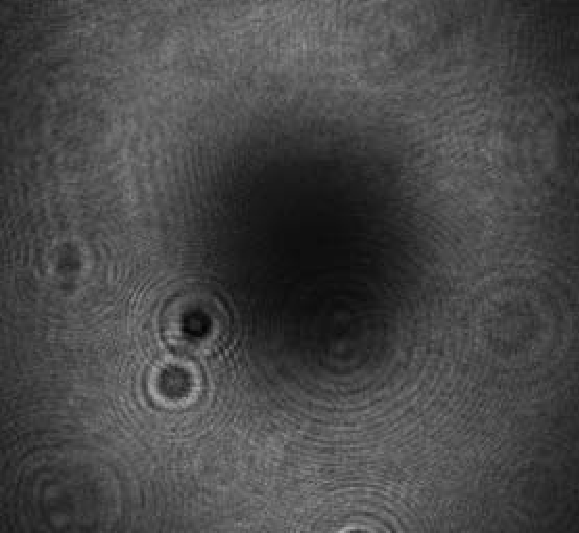
\includegraphics[width=3.5cm]{P3/Sig_M_200_00000_With}}\,
\subfloat[$\Iin \approx \ttfrac{\Isat}{2}$]
{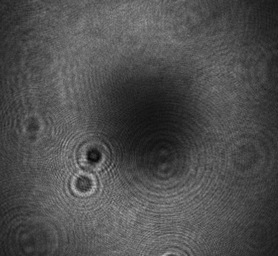
\includegraphics[width=3.5cm]{P3/Sig_M_016_00000_With}}\,
\subfloat[$\Iin \approx 3\,\Isat$]
{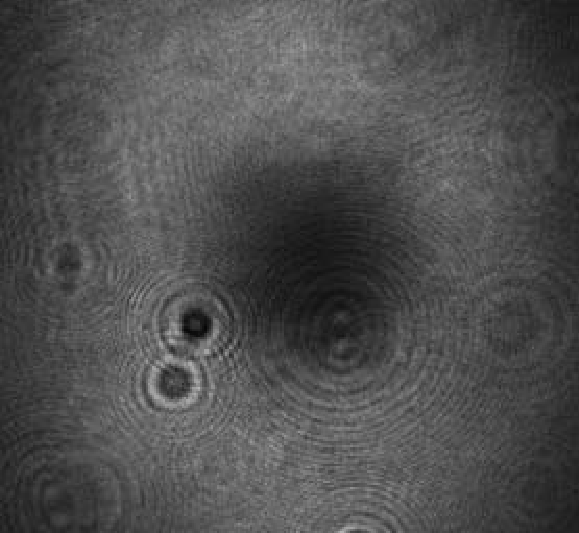
\includegraphics[width=3.5cm]{P3/Sig_M_004_00000_With}}\,
\subfloat[$\Iin \approx 10\,\Isat$]
{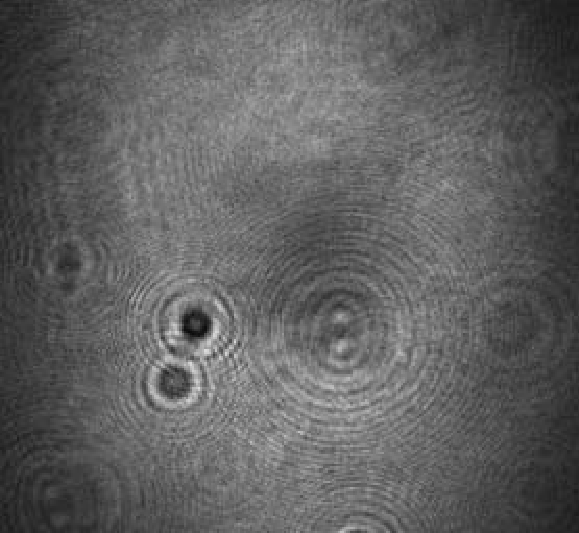
\includegraphics[width=3.5cm]{P3/Sig_M_001_00000_With}}
\CaptionFigs{Représentation de l'absorption du faisceau laser pour différentes intensités incidentes. Celles-ci correspondent à (a) $\Iin = \mWpcmc{0.09}$, (b)$\Iin = \mWpcmc{1.1}$, (c) $\Iin = \mWpcmc{4.5}$, (d) $\Iin = \mWpcmc{18}$.
Les temps d'expositions du capteur CCD sont variés respectivement de \micros{50} à \nanos{250}. Nous ne représentons dans chaque cas que l'image en présence du \nat (voir la~\autoref{sec:ipafas}). 
On constate que le nuage absorbe une grande fraction de la lumière quand celle-ci est peu intense (a). Plus l'intensité incidente $\Iin$ est élevée, plus la fraction de lumière traversant le nuage est élevée. Sur l'image (d), le nuage absorbe moins de la moitié de la lumière incidente.
%Notons que les autres images (\termetech{sans nuage} et \termetech{de fond}) sont indispensables pour le traitement décrit dans cette sous-section, mais ne présentent pas d'interet particulier.
}
\label{fig:PleinImagesNuage}
\efigh

%\AjouteLigne
%\AjouteLigne
\casse

\noindent L'objectif de cette procédure est d'obtenir différentes images d'absorption pour lesquelles les deux termes de l'expression~\nref{eq:DensColAbsHighIntResonance}:
\[
\Imperf \, \Ln{	\frac{\Iin}{\Iout}	}
%\]
\text{~~~et~~~}
% et 
%\[
\frac{\Iin - \Iout}{\Isat}
\virguleformule
\] 
 interviennent \emph{avec des poids différents}. En effet on peut montrer que:
\begin{itemize}
	\item le premier terme (en logarithme) est une fonction décroissante%
	\footnote{Pour montrer que le terme en logarithme est une fonction décroissante de $\Iin$, il faut tenir compte du fait que $\Iout$ dépende de $\Iin$. Qualitativement, on voit bien que si $\Iin$ est très faible, la lumière est absorbée suivant la loi de Beer-Lambert (le logarithme est de l'ordre de quelques unités), alors que si $\Iin$ est très élevée, l'absorption sature (le logarithme tend vers $0$).} de l'intensité incidente $\Iin$,
	\item l'autre terme (différentiel) est une fonction croissante de l'intensité incidente $\Iin$.
\end{itemize}
\Resultat{
L'idée est alors la suivante : 
\begin{itemize}
	\item pour un même \n, nous aurons différentes images, qui doivent cependant toutes permettre de calculer la même \pro par l'expression~\nref{eq:DensColAbsHighIntResonance}, puisqu'elle ne fait aucune hypothèse quant à l'intensité incidente du laser,
	\item or les deux termes de cette expression interviennent avec des poids différents, et \emph{seul le premier} fait intervenir le \pdc $\Imperf$.
\end{itemize}
On en déduit qu'il n'y a qu'une valeur possible pour $\Imperf$ qui permette de concilier toutes les images.
}
%
Pour illustrer ce propos, supposons, l'espace d'un instant, que $\Imperf=1$, \cad que la situation expérimentale corresponde précisément au cas théorique d'un atome à deux niveaux soumis à une onde laser résonnante. 
\inlinefig{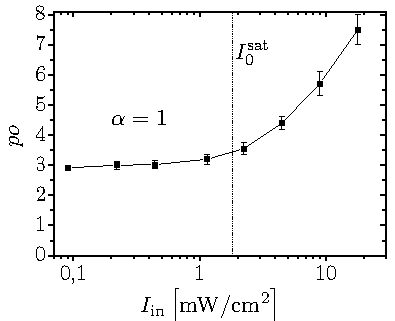
\includegraphics{P3/AllureAlphaEgal1}}\label{fig:AllureAlphaEgal1}\noindent%
Dans ce cas, les images qui font l'objet de la figure~\nref{fig:PleinImagesNuage} ne donnent pas toutes la même valeur de la \pro. La figure ci-contre représente la \pro $\OptProfMax$ du \n %qui correspond au centre du nuage%
%
\footnote{Dans notre cas, la valeur maximale de la \pro est obtenue en ajustant une fonction gaussienne à deux dimensions $G\xy$ sur les données $\OptProf\xy$. La forme du nuage dont il est question ici se prête en effet bien à cette fonction d'ajustement. L'amplitude de la gaussienne donne la valeur $\OptProfMax$.}
% (là où elle est maximale).
%
%Pour obtenir la \dcol $\denscolxy$ du nuage, les différentes images obtenues sont traitées grâce à l'expression~\nref{eq:DensColAbsHighIntResonance}. Celle-ci \emph{doit} donner le même résultat pour toute la série d'images, puisqu'elle ne fait aucune hypothèse quant à l'intensité incidente du laser%
%\footnote{contrairement à l'expression \vref{eq:DensColAbsorption} relative à l'\ipafas}.
%On constate cependant que la \pro $\OptProf\xyImperf$ du nuage calculée dans le cas idéal ($\Imperf = 1$) est une fonction croissante de l'intensité incidente. Nous représentons ci-contre 
en fonction de $\Iin$, valeur moyenne de l'intensité laser. L'\intsat est repérée par une ligne pointillée. Les barres d'erreur sont obtenues en effectuant chaque mesure une dizaine de fois.
La croissance de la courbe montre que, en supposant $\Imperf = 1$, nous sous-estimons le terme décroissant (en logarithme) de l'expression~\nref{eq:DensColAbsHighIntResonance}. Ceci signifie donc que~$\Imperf > 1$.
\picskip{0}

\casse 

\subsubsection{Ajustement du \pdc}
Afin de déterminer $\Imperf$, nous allons %\sotosay{tester} un nombre arbitraire de valeurs possibles pour ce paramètre. Pour souligner le fait que nous 
 le considérer comme une variable ajustable que nous noterons $\ImperfVarie$.%
 \nome{\ImperfVarie}{Valeur ajustable du \pdc}%
 

\Remarque{
Nous utilisons cette notation afin de ne pas confondre la variable ajustable $\ImperfVarie$ avec la \sotosay{vraie} valeur $\Imperf$. En d'autres termes, $\Imperf$ est la valeur particulière du \pdc sur laquelle doit être ajustée $\ImperfVarie$.
}
%
Comme dans l'exemple précédent (nous avions considéré le cas idéal $\ImperfVarie=1$), nous calculons la \pro $\OptProf\xyImperfVarie$ par l'expression~\nref{eq:DensColAbsHighIntResonance} pour chaque intensité $\Iin$ utilisée.
%, mais en utilisant différents paramètres $\ImperfVarie$. 
Rappelons que $\OptProf$ est une \emph{caractéristique physique du \n} et ne dépend donc pas de la manière dont on pratique la mesure. En d'autres termes, pour toutes les intensités incidentes utilisées, on doit normalement obtenir la même \pro par l'expression~\nref{eq:DensColAbsHighIntResonance}.
%  et calculons la \pro  de l'expression~\nref{eq:DensColAbsHighIntResonance}, et ce, pour chaque image de la série. 
La figure~\nref{fig:PleinAlphaCourbe} représente quelques-unes des courbes ainsi obtenues, en utilisant différentes valeurs pour le paramètres $\ImperfVarie$.
\bfighs
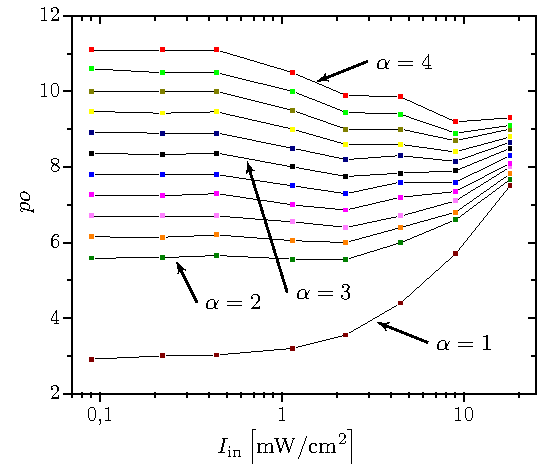
\includegraphics{P3/PleinAlphaCourbe}
\CaptionFigss{Représentation de la \pro $\OptProfMax$ du nuage calculée grâce à l'expression~\nref{eq:DensColAbsHighIntResonance}, en fonction de $\Iin$ (valeur moyenne de l'intensité du faisceau imageur sur le \n). Afin d'améliorer la lisibilité de la figure, les barres d'erreurs n'ont pas été représentées ici.
Chaque courbe correspond à une valeur différente du \pdc $\ImperfVarie$ utilisé lors du calcul par l'expression~\nref{eq:DensColAbsHighIntResonance}. 
%En pratique, une dizaine de valeurs différentes sont prise sur une plage arbitraire. 
Nous utilisons ici les valeurs suivantes pour $\ImperfVarie$ (de bas en haut):  $\ImperfVarie=\val{1}$ (voir la figure~\nref{fig:AllureAlphaEgal1}), puis $\ImperfVarie=\val{2}$ ; $\val{2.2}$ ; $\val{2.4}$ ... $\val{3.8}$ ; $\val{4}$.
}
\label{fig:PleinAlphaCourbe}
\efigh
\Cahier{7,140}

\noindent De manière purement qualitative, on constate sur cette figure que :
\begin{itemizel}
	\item certaines courbes sont décroissantes, laissant supposer que le $\ImperfVarie$ utilisé est trop grand, 
	\item certaines sont croissantes, indiquant que le $\ImperfVarie$ utilisé est trop faible,
	\item l'une de ces courbes ($\ImperfVarie = 3$) varie moins que les autres, approchant le comportement attendu d'une indépendance totale face à l'intensité incidente $\Iin$.
\end{itemizel}

\casse

\noindent De manière à rendre cette analyse quantitative, nous calculons, pour chaque courbe $\OptProfMax(\ImperfVarie)$, l'écart type $\DeltaOP$ des valeurs qu'elle prend. Plus $\DeltaOP$ est faible, plus la courbe est proche du comportement attendu, \cad présentant une indépendance vis-à-vis de l'intensité $\Iin$ utilisée pour la mesure. La figure~\nref{fig:PleinAlphaSTD} représente $\DeltaOP$ en fonction des valeurs de $\ImperfVarie$ utilisées. La valeur $\Imperf$, qui minimise l'écart type, est déduite par ajustement d'une fonction hyperbolique. 
%
\bfighs
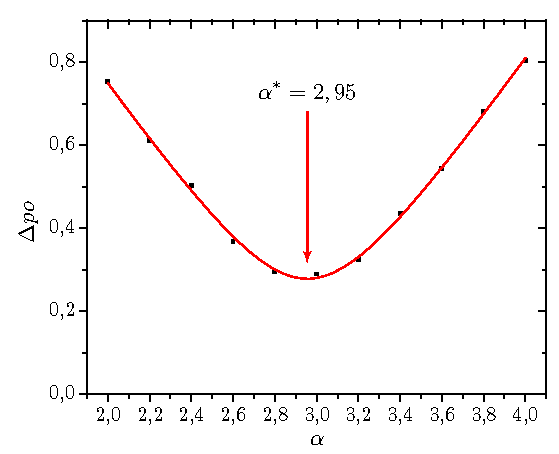
\includegraphics{P3/PleinAlphaSTD}
\CaptionFigs{Écarts types $\DeltaOP$ de chaque courbe de la figure~\nref{fig:PleinAlphaCourbe} en fonction de la valeur de $\ImperfVarie$ utilisée. La présence d'un minimum pour une valeur $\ImperfVarie \equiv \Imperf = \val{2.95}$ est déduite par ajustement d'une fonction hyperbolique (ligne rouge).}
\label{fig:PleinAlphaSTD}
\efigh

Nous déduisons ainsi, dans le cas de notre exemple, $\Imperf = \val{2.95}$, et nous pouvons, grâce à cette valeur, exploiter quantitativement les informations contenues dans les images d'absorption. Dans le cas de notre exemple, nous mesurons une \pro $\OptProfMax = \val{8.4}$ et un nombre d'atomes total $N=\val{3.4E{8}}$.
Nous avons par ailleurs vérifié que le paramètre $\Imperf$ dépend de la polarisation du faisceau imageur.


\subsection{Conclusion}\label{sec:ImageNuageDense}
Nous concluons ce chapitre en présentant des exemples d'images prises et interprétées en utilisant notre protocole d'\ipadrfs. Nous récapitulerons aussi les trois qualités majeures de cette technique.

\subsubsection{Exemples d'images exploitées par notre protocole}
Les figures~\nref{fig:ImageNuageTresDense} et~\nref{fig:PhotosArticleImagerie} présentent deux exemples de \nats denses produits par un \pmobd comprimé. Dans ces cas expérimentaux, le \pdc a été ajusté par la méthode exposée dans la~\autoref{sec:ProtocoleMesureImperf} à une valeur $\Imperf=\val{2.12}$. Nous mesurons ainsi des \pros allant jusqu'à \val{20} (pour la figure~\nref{fig:ImageNuageTresDense}). 
Sur la figure~\nref{fig:PhotosArticleImagerie}, on constate que la structure bimodale résultant de la compression n'est pas apparente lorsqu'on utilise le régime faiblement saturant. Par ailleurs, l'utilisation d'un laser désaccordé ne permet pas d'exploiter l'image obtenue.
\bfighs
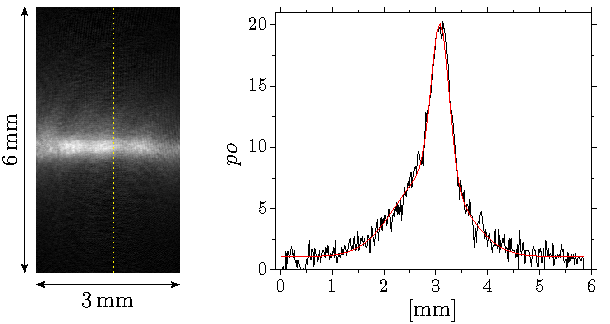
\includegraphics{P3/A_00015AbsorCoupe}
\CaptionFigss{Image représentant la \pro $\OptProf\xy=\seceff\,\denscolxy$ d'un \nat dense produit par un \pmobd comprimé (du fait de la forme longiligne du \n, on n'en distingue qu'une partie sur cette image). Le graphe représente le valeur de la \pro le long de la ligne pointillée. Les \pros élevées excluent l'utilisation de l'\ipafas. Afin d'interpréter l'image, nous ajustons une fonction somme de deux gaussiennes qui permet de caractériser la structure bimodale du nuage (la fonction est représentée en rouge sur le graphe).}
\label{fig:ImageNuageTresDense}
\efigh

\bfighss
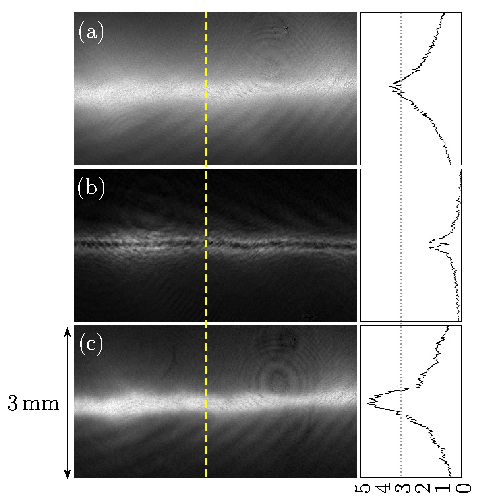
\includegraphics{P3/PhotosArticleImagerie_opt}
\CaptionFigs{Trois mesures de \pro effectuées sur un même \nat comprimé. Sur la droite, on représente le profil de $\OptProf$ le long de la ligne tireté sur l'image. La mesure est effectuée de trois manières différentes: \\
(a) en appliquent le protocole d'\ipafas.\\
(b) un laser désaccordé de $\desac=-3\,\pulsSpont$ est utilisé. L'effet de lentille rend l'image inexploitable.\\
(c) est obtenu en utilisant notre technique d'\ipafos.\\
\emph{Seule cette dernière image met en évidence la structure bimodale} résultant de la compression. La mesure sur (a) ne peut donner de valeurs supérieures à $\approx3$ (ligne pointillée dessinée sur les graphes).}
\label{fig:PhotosArticleImagerie}
\efigh

\casse

\subsubsection{Récapitulatif des avantages de notre protocole}
Récapitulons enfin les principaux atouts de notre protocole d'\ipadrfs:
\begin{ditemize}
	\item le système optique nécessaire pour pouvoir appliquer cette méthode est tout à fait standard et ne nécessite pas de matériel lourd. Il est fort probable qu'un quelconque dispositif permettant d'effectuer des prises d'images par absorption dans le régime de faible saturation puisse être immédiatement adaptable pour mener à bien notre protocole. 
	\vspace{5pt}
	\item l'utilisation d'intensités laser supérieures à l'\intsat permet de contourner les problèmes liés à l'absorption quasi-totale de la lumière laser par un nuage optiquement \termetech{épais} ($\OptProf > 5$). Nous pouvons ainsi observer des \pros très élevées là où l'imagerie basse intensité est inefficace (voir la~\autoref{sec:LimiteIpafas}). Pour pouvoir observer convenablement une \pro $\OptProf$, l'intensité laser nécessaire est typiquement : 
\[
\Ilaser = \frac{\OptProf}{\Imperf} \, \Isat
\pointformule
\]
	\item La détermination du \pdc $\Imperf$ permet d'exploiter de manière quantitative les images par absorption. Il faut d'ailleurs noter que les mesures effectuées sur des \nats \emph{optiquement peu denses} (qui peuvent donc être imagés par la technique usuelle dans le régime faiblement saturant) devraient toujours tenir compte de la valeur du \pdc $\Imperf$. Rappelons en effet que celui-ci intervient dans le calcul de la \dcol (voir l'expression~\nref{eq:DensColAbsHighIntResonance}).
\end{ditemize}







